\documentclass[a4paper, twoside, 12pt]{book}

\usepackage[greek, french]{babel}
%--------------------------
% INPUTENC (encodage du texte)
% FONTENC (positionnement des accents)
%--------------------------
\usepackage[utf8]{inputenc}
%\usepackage{ae,lmodern}
\usepackage[T1]{fontenc}

% Interligne
\usepackage{setspace}

%Pour gérer caractères spéciaux °
\DeclareUnicodeCharacter{00B0}{ }
%Pour les épigraphes
\usepackage{epigraph}
\setlength{\epigraphrule}{0pt}
\setlength{\epigraphwidth}{0.6\textwidth}
 \renewcommand\textflush{flushepinormal}
 \renewenvironment{flushepinormal}{}{\vspace*{-\baselineskip}}
\usepackage{booktabs} % Required for better table rules
% Title page details: 
%--------------------------
% HYPERREF (liens hypertextes et métadonnées)
%--------------------------
\usepackage{hyperref}
\hypersetup{%
colorlinks=true,
linkcolor=black,
urlcolor=blue,
citecolor=black
}

\title{Mémoire de Master 2}
\author{Jean Barré}

%--------------------------
% TOCBIBIND (ajouter la bibliographie dans la Table des matières)
%--------------------------
%\usepackage{tocbibind}
\usepackage[nottoc,notlot,notlof]{tocbibind}
%--------------------------
% Éléments de mise en page (marge de 2,5 cm, alinéa en début de paragraphe 1cm, interligne 1,5)
%--------------------------
\usepackage[a4paper, margin=2.5cm]{geometry}
\usepackage{setspace}
\onehalfspacing
\setlength{\parindent}{1cm}

\usepackage{fancyhdr}
\setlength{\headheight}{28pt}
\renewcommand{\chaptermark}[1]{\markboth{#1}{}}
\renewcommand{\sectionmark}[1]{\markright{#1}}
\pagestyle{fancy}
\fancyhf{}
\fancyhead[LE,RO]{\thepage}
\fancyhead[LO]{\nouppercase{\rightmark}}
\fancyhead[RE]{\nouppercase{\leftmark}}
\renewcommand{\headrulewidth}{0pt}

%--------------------------
% Modules pour gérer les listes
%--------------------------
\usepackage{enumerate}
\usepackage{enumitem}


%--------------------------
% BIBLIOGRAPHIE
%--------------------------
\usepackage[backend=biber, sorting=nyt, style=enc]{biblatex}
\usepackage[autostyle]{csquotes}

%\bibliography{mybibliography.bib}

\addbibresource{biblio/biblio_temp_lit.bib}
\addbibresource{biblio/biblio_temp_tech.bib}

\setcounter{secnumdepth}{5}
\setcounter{tocdepth}{2}

\usepackage[official]{eurosym}
\usepackage{afterpage}
\usepackage{booktabs,xltabular}
%--------------------------
% FIGURES
%--------------------------
\usepackage{graphicx}
\graphicspath{ {./images/} }
\usepackage{float}

% ============================================

\begin{document}

\frontmatter
\begin{titlepage}
\begin{center}

\bigskip

\begin{large}
UNIVERSITÉ PARIS, SCIENCES \& LETTRES
\end{large}

\begin{center}\rule{2cm}{0.02cm}\end{center}

\bigskip
\bigskip
\bigskip
\begin{Large}
\textbf{Jean Barré}\\
\end{Large}
\begin{normalsize}
\textit{Diplômé de licence de Lettres}\\
\textit{Diplômé de licence d'Informatique}\\
\end{normalsize}

\bigskip
\bigskip
\bigskip

\begin{Huge}
\textbf{PRÉDIRE LA CANONICITÉ}\\
\end{Huge}

\bigskip
\bigskip
\begin{LARGE}
\textbf{Étude des dynamiques à grande échelle des
processus de canonisation}\\
\end{LARGE}

\bigskip
\bigskip
\bigskip
\vfill

\begin{large}
Mémoire de deuxième année du master\\
\og Humanités Numériques \fg{} \\
\bigskip
2022
\end{large}

\end{center}
\end{titlepage}

\section*{Résumé}
\addcontentsline{toc}{chapter}{Résumé}
Ce projet interroge le canon littéraire, une notion construite avec les biais de la société et modelée par les réceptions successives. L’objectif de ce rapport est de mettre en lumière l’existence de dynamiques textuelles qui assurent une longévité exceptionnelle à certains ouvrages et menacent au contraire la transmission d’une majorité d’autres. Les méthodes quantitatives du traitement automatique des langues et de l'apprentissage machine nous permettent de mettre au jour une esthétique intrinsèque au canon littéraire. Nous proposons une modélisation statistique de la canonicité avec des résultats prédictifs allant jusqu'à 90\% d'efficacité.


%, avec le contexte des œuvres,
% nous permettent de réaliser des analyses en \textit{lecture distante}\footnote{Franco Moretti. « Conjectures on World Literature », \textit{New Left Review}, 2000. republié dans \cite{moretti_distant_2013}} pour faire l’exégèse des tendances historiques qui caractérisent le canon littéraire par opposition avec les œuvres rejetées par ce dernier.


\medskip

\textbf{Mots-clés: études littéraires computationnelles ; canon littéraire ; classique ; littérature ; stylométrie ; histoire littéraire ; humanités numériques ; lecture distante ; traitement automatique de la langue ; apprentissage machine}

\textbf{Informations bibliographiques:} Jean Barré, \textit{Prédire la canonicité : Étude des dynamiques à grande échelle des
processus de canonisation}, mémoire de master 1 \og Humanités Numériques\fg{}, dir. [Thierry Poibeau, Jean-Baptiste Camps], Université Paris, Sciences \& Lettres, 2021.



\section*{Abstract}
\addcontentsline{toc}{chapter}{Abstract}
This project will interrogate the literary canon, a notion constructed with the biases of society and shaped by successive receptions. The aim of this report is to shed light on the existence of textual dynamics which ensure an exceptional longevity to some works and threaten the transmission of a majority of others. The quantitative methods of natural language processing and machine learning allow us to uncover an intrinsic aesthetic of the literary canon. We propose a statistical modeling of canonicity with predictive results of up to 90\% accuracy.

%, together with the context of the works,

% allow us to carry out analyses in \textit{distant reading}\footnote{Franco Moretti. "Conjectures on World Literature", \textit{New Left Review}, 2000. republished in \cite{moretti_distant_2013}} to exegete the historical trends that characterise the literary canon as opposed to the works rejected by it.

\medskip

\textbf{Keywords: computational literary studies ; canon ; classic ; archive ; literature ; stylometry ; digital humanities ; distant reading ; text mining ; natural langage processing ; machine learning}

\textbf{Bibliographic Information:} Jean Barré, \textit{Predicting canonicity, large scale dynamics of canonization processes}, M.A. thesis \og Digital Humanities\fg{}, dir. [Thierry Poibeau, Jean-Baptiste Camps], Université Paris, Sciences \& Lettres, 2021.


\clearpage
\chapter*{Remerciements}
\addcontentsline{toc}{chapter}{Remerciements}
\markboth{Remerciements}{} 
\bigskip



Je tiens à remercier chaleureusement mon directeur de mémoire Monsieur Thierry Poibeau, pour son enthousiasme pour le projet, sa grande disponibilité, et ses innombrables retours. Je tiens également à remercier mon directeur de mémoire Monsieur Jean-Baptiste Camps pour sa bienveillance, ses réflexions toujours pertinentes et le support technique qu'il m'a apporté. 

J’aimerais aussi remercier Messieurs Simon Gabay et Chahan Vidal-Gorène pour leurs conseils et l’intérêt qu’ils ont montré pour ce travail.

Ce mémoire n'aurait pas été possible sans le soutien de mon amoureuse Marie Delille et mes amis proches, qui m'ont soutenu malgré mes trop longs exposés quotidiens sur le sujet.

Je tiens enfin à remercier mes parents, ma sœur et mon frère pour leurs corrections bienvenues, mais surtout pour leur amour et leur soutien indéfectible.


% table des matières
\addcontentsline{toc}{chapter}{Table des matières}
\tableofcontents

\mainmatter

\part*{Introduction}
\addcontentsline{toc}{part}{Introduction}
\markboth{Introduction}{Introduction}

\vspace*{\fill}
\epigraph{Les plus beaux livres sont écrits dans une sorte de langue étrangère.}{\textit{Marcel Proust, Contre Sainte Beuve, 1954}}
\epigraph{On peut aussi construire un modèle du \textit{processus de canonisation qui conduit à l'institution des écrivains}, à travers une analyse des différentes formes que le panthéon littéraire a revêtues, aux \textit{principes de classement} eux-mêmes \textit{pré-construits}.}{\textit{Pierre Bourdieu, Les règles de l'art, 1992}}

\vfill\clearpage
%abrupt

Stendhal est aujourd'hui considéré comme un auteur incontournable de la littérature française. Pourtant, la présence de cet auteur majeur dans la conscience collective n'a pas toujours été évidente. La renommée de son oeuvre n'arrive que longtemps après sa mort. Quels processus ont joué un rôle dans la canonisation de cet auteur ? La reconnaissance des romans de Stendhal est un exemple parmi les milliers de romans du XIXème et du XXème siècle, alors pourquoi et comment se démarquent-ils des autres ouvrages laissés à l'abandon littéraire ? 

L'ensemble des auteurs que l'on appelle \textit{les classiques} forme le canon littéraire. Nous pouvons définir ce dernier comme le résultat d'une tradition sélective\footcites{pollock_differencing_1999} dont la mémoire collective a gardé le souvenir parce qu’elle leur confère un statut prééminent.

%Nous voulons décrire et comprendre les mécanismes derrière cette filtration temporelle, qu’ils soient liés à des politiques culturelles ou à des critères autonomes, d’ordre esthétique et critique

Historiquement, les études sur les processus d'attribution de la valeur littéraire se sont intéressées aux contextes dans lesquels étaient produites les oeuvres, et aux processus de canonisation des auteurs et de leurs oeuvres. Dans \textit{Les règles de l'art}\footcites{bourdieu_les_1992}, un ouvrage majeur concernant notamment le prestige littéraire, Pierre Bourdieu montre que les mécanismes derrière la distribution du prestige littéraire sont fondés sur des facteurs appartenant aux contextes des oeuvres. Ces facteurs sont liés entre autres aux dynamiques de pouvoir au sein du champ littéraire. Les contextes de production expliqueraient deux \enquote{modes de vieillissement} des auteurs, d'une part ceux consacrés par la critique et l'enseignement et d'autre part ceux voués à une \textit{mort} littéraire rapide.

Le prestige littéraire est donc une notion complexe à envisager et les mécanismes derrière cette filtration temporelle sont nombreux, qu'ils soient liés à des politiques culturelles ou à des critères autonomes, d'ordre esthétique et critique.

Nous voulons, dans ce mémoire, revenir aux textes et à leur contenu. Notre hypothèse est de dire qu'il y a une esthétique particulière dans le canon, et qu'on peut la détecter et la décrire. Notre travail consistera à présenter les différents éléments mis en place pour prédire la \textit{canonicité} avec le contenu textuel des ouvrages. Nous nous fonderons sur des outils du traitement automatique des langues, de la stylométrie et des techniques d'apprentissage machine pour caractériser cette notion de canon littéraire.

Les humanités numériques, et plus précisément les études littéraires computationnelles, s'inscrivent dans une nouvelle approche de compréhension de la production culturelle des siècles passés. Un des concepts sur lequel se fonde cette nouvelle approche est le \textit{\enquote{distant reading}}\footnote{Franco Moretti. « Conjectures on World Literature », \textit{New Left Review}, 2000. On notera une synthèse des écrits autour de cette notion dans un ouvrage dédié au \textit{\enquote{distant reading}}.\cite{moretti_distant_2013}.}, théorisé par Franco Moretti dans les années 2000. Cette \textit{\enquote{lecture distante}} a pour ambition d'explorer le passé littéraire avec des méthodes scientifiques sur des corpus massifs et numérisés. 

Le nouveau paradigme ouvert par le numérique en stylistique et en histoire littéraire est précisément de dépasser la seule étude du canon littéraire, qui est composé simplement quelques centaines d'oeuvres en opposition avec les milliers d'oeuvres rejetées par celui-ci. Un des constats posé par Ted Underwood\footnote{\cite{underwood_distant_2019}, chap. 1 p 1 - 33} est que les études littéraires ne connaissent pas vraiment les grandes lignes structurantes de l'histoire littéraire. En effet, la discipline s'est focalisée des années durant sur une poignée d'oeuvres du canon littéraire. Cette sélection est assimilable pour certains chercheurs à un \textit{\enquote{abattoir littéraire}\footcites{moretti_slaughterhouse_2000}}. Ce dernier contient selon Moretti une histoire bien différente de celle contenue dans les canons académiques, et le \textit{\enquote{distant reading}} peut permettre de prendre en considération ces milliers de volumes oubliés. 

L'utilisation de techniques du traitement automatique des langues (TAL) pour l'analyse de corpus littéraires a donné lieu à de nombreuses études, que ce soit pour la modélisation du genre\footnote{Ted Underwood, \textit{The life spans of genres} in \cite{underwood_distant_2019}, p 34 - 67}, du suspense\footcites{piper_narrativity_2021}, des thèmes\footcites{jockers_significant_2013}, ou de la paternité des oeuvres\footcites{cafiero2021psyche}. Il s'agit d'explorer des motifs et des tendances historiques sur la longue durée \footcites{braudel_mediterranee_2017}, à partir de corpus littéraires massifs et numérisés. C'est un domaine de recherche très actif aux États-unis et en Europe, mais beaucoup moins en France, bien qu'il existe également de puissants outils du TAL pour le français, ainsi que des corpus accessibles.

Cette approche ne vise à effacer ni les siècles de lecture proche ni la subjectivité du chercheur. Elle permet d'élargir la focale pour interroger nos savoirs critiques hérités mais aussi pour en produire de nouveaux. 

Ce mémoire s'inscrit nécessairement dans une étude de la réception et un temps sera consacré à recueillir des méta-données pour construire un canon littéraire que l'on questionnera dans les textes. L'objectif premier est d'enrichir un corpus avec le contexte social de production et de réception. 

Dans un premier temps, nous définirons les enjeux de recherche autour de la notion de prestige littéraire. Dans un second temps, nous construirons un canon littéraire fondé sur une multiplicité de facteurs diagnostiqués par la recherche en sociologie et en histoire littéraire. Dans un troisième temps, nous modéliserons la notion de canon littéraire pour mettre au jour une esthétique propre. Enfin, un retour qualitatif sur les inférences statistiques de nos différents modèles sera nécessaire pour caractériser avec plus de finesse cette esthétique canonique.
\part{Préliminaires}

\chapter{Les modalités du canon littéraire}
%wrong title 

\section{\textit{Canon} et \textit{classiques} de la littérature}

Nous utiliserons dans ce mémoire la notion de \textit{canon littéraire} dans le sens où ce dernier est composé d'ouvrages \textit{classiques}, ou d'auteurs \textit{classiques}. 

Le mot canon vient du grec \enquote{\foreignlanguage{greek}{Κανων}} qui signifie \enquote{roseau} ou \enquote{tige}, littéralement \enquote{droit comme une tige de roseau} \footnote{William Marx,  cours au collège de France, \url{https://www.college-de-france.fr/site/william-marx/course-2021-04-13-14h30.htm}} utilisé comme un instrument de mesure. Avec le temps le terme prend le sens de \enquote{règle} ou de \enquote{loi}, et c'est avec cette signification qu'il arrive dans les langages européens modernes. C'est au quatrième siècle après JC\footnote{John Guillory, \enquote{Canon} in \cite{lentricchia_critical_2012},  p.233-245}, avec le canon biblique, que le mot prend le sens actuellement utilisé dans les études littéraires. L'Église instaure une liste de textes formant les Saintes Écritures. Le canon avait alors une valeur d'autorité qui permettait à l'Église de contrôler un récit commun pour la postérité.

%le canon comme bibliothèque mentale collective. cf William Marx

La notion a été introduite dans les études littéraires pour désigner les syllabus des universités et les textes qui y étaient étudiés. Selon certains chercheurs, le canon est nécessaire à l'enseignement de la littérature : \enquote{L'étude institutionnelle de la littérature est inconcevable sans un canon. Sans canon, sans corpus ou syllabus de textes exemplaires, il ne peut y avoir de communauté interprétative.}\footnote{\cite{felperin_beyond_1985}, les traductions des citations ont été réalisés par mes soins}. Le canon est ainsi l'ensemble des textes sur lesquels se fonde la discipline et la recherche en littérature. Pour Pascale Casanova, le canon \enquote{incarne la légitimité littéraire elle même, c'est à dire ce qui est reconnu comme \textit{la littérature}, et qui servira d'unité de mesure spécifique}\footcites{casanova_republique_2008}.  

W. Harris distingue différentes fonctions du canon littéraire\footcites{harris_canonicity_1991} : Il permet de \enquote{fournir des modèles, de transmettre l'héritage de la pensée, par la provision de savoirs culturels nécessaires pour interpréter les textes du passé}. Le canon crée des cadres de référence communs pour faire société par identification à un ensemble de mythes et de textes sacrés. Un des problèmes soulevés par ce genre d'approche du canon est que si l'on se penche sur les listes des grands auteurs qui les composent, on trouvera très peu de femmes, et encore moins d'auteurs non blancs, ou de classe sociale défavorisée\footcites{guillory_cultural_1998}. Les processus de formation du canon littéraire sont souvent exclusifs, et il faudrait déconstruire les préjugés sur lesquels se fonde le canon.

Les polémiques sur le canon littéraire ont été particulièrement virulentes dans les campus universitaires étasuniens à partir des années 1980. La synthèse d'Eric Fassin\footcites{fassin_chaire_1993} est à cet égard fort instructive. Deux camps s'affrontent, avec d'un côté les défenseurs du canon (compris comme la quintessence de la tradition littéraire occidentale\footcites{bloom_western_1994}) au nom des valeurs universelles qu'il incarne. De l'autre côté, ses détracteurs, qui relèvent les conditions sociologiques, géographiques, idéologiques et culturelles de la production des critères de définition et de sélection du canon littéraire\footcites{harder_deconstruire_2013}. 

En France, la notion de canon n'est pas si répandue et doit son existence aux polémiques venant d'outre-Atlantique. C'est le terme \textit{classique} qui est utilisé, et qui n'est d'ailleurs pas dédié uniquement à l'espace littéraire. Le nom \textit{les Classiques} désigne aujourd'hui les grands écrivains de la littérature française, mais cela n'a pas toujours été le cas.

Le mot \textit{classique} vient du vocabulaire de la richesse et de la propriété. Du latin \textit{classicus}, signifiant \enquote{citoyen de la première classe}\footnote{Trésor de la langue française informatisé ; https://atilf.fr/ressources/tlfi}. L'adjectif \textit{classique} prend son sens de jugement esthétique au XVII\ieme siècle, où il signifie ce qui mérite d'être copié ou de servir de modèle. A la fin du XVII\ieme siècle, la signification dérive et prend le sens de ce qui était enseigné en classe. Au cours du XVIII\ieme siècle, le terme désigne les auteurs antiques grecs ou latins. 

Finalement au cours du XIX\ieme siècle, on appelle \textit{classiques}, par opposition aux auteurs romantiques contemporains, les auteurs du temps de Louis XIV et cette époque comme le classicisme français\footcites{viala_quest-ce_1993}. Ainsi, dans son sens le plus restreint, le \textit{classique} désigne les auteurs de théâtre du XVII\ieme siècle, considéré comme le grand siècle de la littérature française puisque cette période littéraire s'est le plus rapproché de la perfection antique.

L'enjeu du terme \textit{classique} se joue au niveau de la réception. Ce n'est pas l'auteur qui choisit d'être classique, c'est l'institution scolaire ou la critique, et ses représentants, qui choisissent et émettent le jugement esthétique et politique de son appartenance au cercle des \textit{classiques}.

Sainte-Beuve, critique et écrivain français conservateur du milieu XIX\ieme siècle nous donne un bon échantillon de la perception des classiques au XIX\ieme siècle :
\begin{displayquote} \enquote{Un vrai classique, comme j'aimerais à l'entendre définir, c'est un auteur qui a enrichi l'esprit humain, [...] qui a découvert quelque vérité morale non équivoque, [...] qui a parle à tous dans un style à lui et qui se trouve aussi celui de tout le monde, dans un style [...] nouveau et antique, aisément contemporain de tous les âges.}\footnote{Sainte-Beuve, \textit{Causeries du lundi}, cité dans\cite{compagnon_sainte-beuve_1995}}
\end{displayquote}
Plusieurs éléments sont intéressants. La notion de style - que nous discuterons plus tard dans cette partie - apparaît centrale pour définir le classique. Sainte-Beuve ne nous aide pas en présentant avec deux oxymores le style classique, qui serait à la fois personnel et commun, \enquote{nouveau et antique}. Il y a une forme de sacralisation du classique, qui est selon Sainte-Beuve un idéal littéraire que peu d'écrivain ont atteint. Sainte-Beuve essentialise le classique en le rapprochant de la notion de vérité, et justifie ainsi la hiérarchie entre les classiques et les autres.

% Ce jugement de l'esthétique supérieur du style classique est une forme de sacralisation du classique /qui met à distance la littérature contemporaine de la consécration du classique./

\section{Le canon et l'enseignement}

La supériorité esthétique mise en avant par Sainte-Beuve n'est pas suffisante pour expliquer les différents processus de canonisation des auteurs. La relativité du jugement esthétique des critiques ne permet pas d'expliquer la stabilité du canon littéraire. 

C'est dans l'enseignement de la littérature que l'on peut constater les dynamiques de construction et de modification du canon littéraire français. L'institution scolaire est un des lieux majeurs où le canon s'élabore. En effet, elle produit des panthéons d'auteurs et de textes, souvent sous la forme de morceaux choisis\footcites{jey_litterature_1998} pour éduquer des générations d'écoliers. Dès la première liste nationale de 1803, le canon des auteurs français est constitué. Il est repris ensuite pour être diffusé grâce au système scolaire centralisé.

L’institution scolaire construit une représentation de la littérature qui lui est propre. Elle en détermine le bon usage, avec des découpages chronologiques (périodisations, écoles, générations), une utilisation de catégories (romantisme, naturalisme, surréalisme), et enfin l'élaboration d’un canon par une sélection d’auteurs. Ces classiques sont le fruit d’une sélection particulièrement étroite. Ils sont présentés comme des modèles, véhiculant une norme esthétique particulière. C'est cette norme qui nous intéresse et que nous voulons repérer quantitativement.

Le canon littéraire construit par l'institution scolaire devient ainsi matrice de formes spécifiques en tant qu'il est le représentant de ce qui est considéré comme de la \textit{bonne} littérature. Pourtant le canon n'est pas monolithique et s'ouvre au cours du temps. Les garants du bon ordre littéraire (l'institution scolaire et, dans une moindre mesure, la critique) nourrissent et ouvrent le canon sous la pression et l'usure du temps aux oeuvres qui semblent le plus en accord avec une certaine idée de la littérature. 

\section{Un canon politique}

Le canon littéraire porte une dimension politique, tant dans sa construction que dans ce qu'il représente en tant que tel. Selon Alain Viala, les auteurs retenus dans le canon \enquote{remplissent une fonction d’identification culturelle}\footcites{viala_quest-ce_1993}, c'est à dire qu'ils représentent le socle commun de la construction culturelle d'une nation. Dans le contexte français, l'évolution du canon littéraire est le témoin de la légitimation et de l'affirmation d'une langue et d'une culture française par rapport au latin. La première liste institutionnelle d'auteurs de 1803 associe un auteur grec ou latin à un auteur français du XVII\ieme siècle. Avec la structuration et la centralisation du système scolaire sous la troisième république, le canon se cristallise et devient un objet politique\footcites{compagnon_troisieme_1983}. La littérature dans l'enseignement, associée à un canon littéraire, se trouve investie d'un rôle d'éducation des masses et de diffusion de valeurs nationales. On peut trouver un exemple dans le canon des agrégations, qui est \enquote{ramassé autour de ce qui semble incarner les valeurs nationales}\footcites{jey_canon_2014}. Différentes réformes de l'enseignement scolaire ont façonné le canon et la façon d'enseigner la littérature au cours du temps.

Après cette première ouverture du canon littéraire, ce dernier a longtemps été la chasse gardée des auteurs du XVII\ieme siècle, et très peu de genres littéraires étaient représentés. Seul le théâtre et la poésie étaient les genres autorisés, puisqu'ils étaient les garants d'un classicisme formel, modèle d'ordre, de clarté, le tout dans un équilibre et une harmonie parfaits.

A la fin du XIX\ieme siècle, la société évoluant vers une laïcisation des moeurs sociales, l'enseignement de la littérature fait face à des difficultés. Gustave Lanson, célèbre historien et critique littéraire, le constate : 
\begin{displayquote} \enquote{C'est une absurdité de n'employer qu'une littérature monarchique et chrétienne à l'éducation d'une démocratie qui n'admet point de religion d'Etat.}\footnote{Gustave Lanson, «L'étude des auteurs français», Revue universitaire, 1894}
\end{displayquote}

Pour G. Lanson, la République doit se doter de nouveaux \enquote{textes sacrés}\footcites{compagnon_demon_1998}, et le canon littéraire doit s'ouvrir aux écrivains et aux genres littéraires contemporains. Les missions de la littérature sont alors de moraliser les moeurs sociales et de fabriquer un consensus national. Le roman entre ainsi au panthéon de la littérature, et avec lui la plupart des auteurs romanesques considérés encore aujourd'hui comme des classiques de la littérature française. 

%\enquote{C'est un genre littéraire aussi jeune que l'idée de nation, le roman, qui va à la fois servir de modèle narratif pour les premières élaborations savantes d'histoires nationales et de formidables vecteur de diffusion d'une vision nouvelle du passé}\footcites{thiesse_fabrique_2019}.

Lors de la poussée des nationalismes du début du XX\ieme siècle, la littérature doit affirmer l'unité voire la supériorité culturelle de la France. Ces processus ont été étudiés par Anne-Marie Thiesse dans son livre \textit{La fabrique de l'écrivain national : entre littérature et politique}. 
\begin{displayquote}\enquote{La nationalisation de l'état passe au premier chef par un intensif travail d'éducation de masses, visant à inculquer dans l'ensemble de la population le sentiment d'appartenance commune}\footcites{thiesse_fabrique_2019}. \end{displayquote}

Ainsi, le canon littéraire incarne les fondements du récit national. Il peut être vu comme la construction politique de la culture nationale. C'est d'ailleurs un paradoxe que souligne Pascale Casanova dans son livre \textit{La république mondiale des lettres}\footcites{casanova_republique_2008}. Les cultures européennes se fondent sur des canons nationaux, tout en revendiquant les valeurs transnationales et universelles de ces derniers, qui prendraient racine dans un passé lointain des antiques grecs et latins.


\section{Le style et les classiques}
La construction du canon littéraire est éminemment politique, sa mise en place et sa diffusion relevant de politiques culturelles de mise en avant d'une littérature spécifique, censée porter les valeurs des régimes successifs de l'histoire de France. Les architectes du canon ont fondé leur sélection sur des critères linguistiques. Ils ont sélectionné ce qui, selon eux, représentait le meilleur usage de la langue française. Le classique est un modèle de style, et c'est pour cela qu'il est enseigné. Si nous pouvons questionner cette sélection en tant qu'elle lui donne un aspect arbitraire, le jugement esthétique étant par nature relatif, nous ne pouvons pas l'écarter complètement.

On peut définir le style comme \enquote{l'ensemble des traits expressifs qui dénotent l'auteur dans un écrit}\footnote{ Trésor de la Langue Française informatisé, \url{http://stella.atilf.fr/}}. En littérature, on assimile souvent le \textit{style} à l'expression de la singularité de l'auteur, en tant qu'il s'écarte de la \textit{norme}. Pour Georges Molinié, grand stylisticien, \enquote{Il n'y a de style que dans la mesure où des régularités dans le choix permettent de caractériser une écriture}\footcites{molinie_quest-ce_1994}. Le style est un ornement formel, qui est propre à chaque auteur. 



Toujours selon Georges Molinié, les qualités stylistiques des classiques pourraient expliquer leur filtration temporelle : 

\begin{displayquote}
\enquote{Dans la masse des romans et des pièces de théâtre, très peu, [...] sont encore lus de nos jours : l'invention et la gestion des situations dramatiques sont bien moins en cause que la qualité, la force, l’éclat d’écriture. C’est d’abord cette différence stylistique qui a séparé Pradon de Racine ; c’est la phrase de Madame de La Fayette qui a durablement séduit, parmi d’autres écritures effectives, indépendamment des atavismes ou des ruptures de la composition et de l’invraisemblable des situations. [...] Il est difficile de nier cette primauté du style.}\footcites{molinie_style_1996}
\end{displayquote}

La pérennité du canon littéraire peut s'expliquer par la \enquote{primauté du style} présente dans les \textit{classiques} de la littérature. La langue littéraire, que l'on pourrait définir comme la langue des écrivains, se caractérise par son style, en opposition à la langue de tous les jours, qui manque de style. 

Il faudrait revenir sur notre définition du style, et à la tension qui existe entre norme et style. On a vu que le style était traditionnellement vu comme l'expression d'une singularité, c'est à dire d'un idiolecte propre à un auteur. Le style peut aussi être vu comme une généralité, une langue littéraire, c'est à dire un sociolecte utilisé par les écrivains. Selon la formule de Gilles Philippe, la littérature, au sens du canon littéraire, est un \enquote{conservatoire consacrant la norme et un laboratoire célébrant la liberté du locuteur\footcites{philippe_langue_2009}}. Le style est indissociable de ces deux aspects, mais le premier a longtemps été minimisé, au profit du second, par les études stylistiques. 
%p30

Le style présent dans le canon littéraire serait \enquote{une norme étalon à partir de laquelle l'on attribue ou l'on refuse une valeur esthétique à une production langagière}\footcites{philippe_pourquoi_2021}. Il y aurait une norme stylistique haute dans le canon littéraire; c'est cette norme que nous voulons détecter quantitativement. Les méthodes quantitatives semblent les mieux adaptées pour envisager l'ensemble des caractéristiques qui forment l'esthétique de la langue littéraire, ou plus simplement, l'esthétique canonique.
%p63

Le style est une notion que les études quantitatives ont abordé. On peut notamment présenter l'article de Herrmann et al, \enquote{Revisiting style, a key concept in literary studies}. Ces chercheurs ont proposé une définition du style compatible avec les méthodes quantitatives : \enquote{Le style est une propriété du texte constitué par un ensemble de caractéristiques formelles, pouvant être observées quantitativement ou qualitativement}\footcites{BerenikeHerrmann2015RevisitingSA}. La puissance de calcul et l'étude de grand corpus dans le cadre des études littéraires computationnelles peut aider à désingulariser la notion de style. Nous proposons, dans ce mémoire, d'étudier le style comme un phénomène collectif, qui caractériserait l'esthétique spécifique du canon littéraire.

Dans le prochain chapitre, nous verrons comment définir l'approche des études littéraires computationnelles pour appréhender des concepts littéraires tels que celui du style.

%faisceaux - ensemble de traits stylistiques

%\enquote{Pour faire vite, on peut dire que, pendant la première moitié du XXe siècle on a ramené la question de la littérature à celle de la langue littéraire et celle de la langue littéraire à celle de la grammaire, considérée comme charpente des productions langagières. [...] La grammaticalisation de l'ensemble des discours sur la littérature a provoqué l'avènement d'un concept nouveau, [...], celui de "littérarité", qui repose sur l'idée d'une spécificité partielle ou complète du discours littéraire face aux discours non littéraire. En mettant au cœur du débat la question de la grammaire, on passait en effet de la définition humaniste de la littérature comme corpus à une définition formaliste de la littérature comme pratique de la langue}\footcites{philippe_sujet_2002}Gilles Philippe, Le moment grammaticale de la littérature française, 1890-1940, p15

%C'est à partir des années 1850 que semble s'être progressivement imposée en France l'idée selon laquelle la langue des écrivains ne pouvait plus être ramenée à la langue commune. L’idiolecte c’est le style sans la signification, et le style, l’idiolecte en tant qu’il peut faire l’objet d’une interprétation.

%Antoine Albalat : La décomposition du style doit être placée en première ligne dans les études critiques, parce qu'elle est \footnote{\textit{Ouvriers et procédés}, p27-28, cité dans \cite{philippe_reve_2013}, p99}



\chapter{Approches quantitatives}

\section{La mesure dans les études littéraires}

%histoire ancienne -> sacy ? dray ? cours stylométrie ? mais développements récents:

Grâce aux progrès de l'informatique et du traitement du langage naturel, l'utilisation d'approches statistiques et mathématiques dans le domaine des études littéraires a considérablement augmenté ces dernières années. 

La notion de \textit{\enquote{distant reading}}\footnote{Franco Moretti. « Conjectures on World Literature », \textit{New Left Review}, 2000. On notera une synthèse des écrits autour de cette notion dans un ouvrage dédié au \textit{\enquote{distant reading}}.\cite{moretti_distant_2013}.}, définie en introduction n'est finalement qu'une nouvelle approche de description et de production de savoirs empiriques en histoire littéraire. 

Ce nouveau champ de recherches permet d'augmenter la focale en prenant en compte la production littéraire dans un ensemble le plus grand possible. Cela permet de comprendre les contrastes entre des oeuvres tirées de différentes périodes ou de différents contextes sociaux. 

Franco Moretti et le laboratoire littéraire de Stanford\footnote{https://litlab.stanford.edu/} ont contribué à développer cette nouvelle approche des textes littéraires fondée sur la mesure et le calcul de fréquences d'éléments du texte. Leurs pamphlets 1, \enquote{Quantitative Formalism : an Experiment}\footcites{allison_quantitative_2011}, 6, \enquote{"Operationalizing” : or, the function of measurement in modern literary theory}\footcites{moretti_operationalizing_2013} et 12, \enquote{Literature, Measured}\footcites{moretti_literature_2016} conceptualisent le rôle de la mesure pour appréhender des objets culturels. Ces pamphlets fondent une discipline, les études littéraires computationnelles.

Ces dernières modifient l'approche conceptuelle de l'objet d'étude des analyses littéraires traditionnelles. Un roman n'est plus vu comme un objet physique singulier, mais plutôt comme un agrégat de signes caractéristiques et quantifiables, dont l'ensemble ne forme qu'un échantillon parmi un corpus de milliers d'autres ouvrages. Mark-Algee Hewitt, un chercheur du domaine, souligne que \enquote{l'enjeu de cette transformation est donc notre compréhension du roman lui-même : ce qu'il est, les informations qu'il contient et ce qu'il peut faire en tant qu'objet littéraire et critique}\footnote{\cite{algee-hewitt_novel_2018}}. Le roman est ainsi envisagé comme un ensemble de données, dont la signification mathématique peut nous apprendre des éléments critiques sur un auteur, un genre littéraire ou même un espace culturel. 

Cet examen systématique des données contenues dans les textes écrits est conceptualisé par Matthew L. Jockers comme une analyse à l'échelle macroscopique\footcites{jockers_macroanalysis_2013} de la littérature. Cette approche \textit{macro-analytique} permet de comprendre \enquote{le degré auquel la littérature et les auteurs individuels qui la fabriquent répondent ou réagissent aux tendances littéraires et culturelles}. C'est une nouvelle manière de décrire la position de l'écrivain dans le champ littéraire. 

Avec ces nouvelles méthodes, le chiffre et la mesure prennent ainsi une influence particulièrement importante. Ted Underwood explicite leur rôle : \enquote{Les chiffres ne sont pas plus objectifs que les mots. Ils ne sont que des signes qui permettent aux observateurs humains de se débattre avec des questions de degré. Nous avons besoin de chiffres pour comprendre les longues chronologies littéraires}\footcites{underwood_why_2018}. Le chiffre permet de manipuler de grands ensembles de données et de chercher du sens face à la quantité énorme de textes écrits. Le livre d'Andrew Piper - \enquote{Énumérations\footcites{piper_enumerations_2018}} - pose la question des implications de la conception de la littérature comme \textit{quantité}. La multiplicité des possibilités des analyses et la quantité massive de données imposent au chercheur une rigueur scientifique.

% citer cultoromics ? approche pas forcément idiote
La méthode à l'oeuvre ne consiste pas à lancer des calculs exploratoires sur de grands ensembles de données, trouver des motifs de répétitions et d'en tirer les conclusions qui en découlent. Au contraire, elle se fonde sur des hypothèses et des savoirs historiques pour les questionner dans les textes. Les nouvelles méthodes que nous avons décrites fonctionnent en tandem avec la théorie littéraire et l'histoire littéraire. Mettre de côté les immenses savoirs hérités de l'analyse littéraire traditionnelle serait contre-productif et réduirait les capacités d'interprétation des études computationnelles. 

\section{La modélisation en études littéraires}

Dans la dernière décennie, le champ des humanités numériques a pu profiter des grands progrès des méthodes quantitatives. En effet, s'éloignant de la mesure de variables ou de fréquences d'occurrences dans les textes, les recherches actuelles utilisent désormais des modèles statistiques pour appréhender des concepts littéraires. Les recherches sont passées de méthodes statistiques descriptives à des méthodes prédictives de modélisation.

Dans ce mémoire, nous mettons en oeuvre ce genre de techniques et nous voulons ici préciser les modalités de leur emploi. L'introduction de l'apprentissage machine dans les processus de réflexion des sciences humaines va au delà des mesures en lecture distante. Selon Richard J. So, \enquote{La lecture à distance est innovante parce qu'elle a introduit non seulement des \enquote{données} ou des \enquote{algorithmes} dans les études littéraires, mais aussi, et surtout, la modélisation quantitative comme forme de raisonnement et d'analyse}\footcites{so_all_2017}. La modélisation statistique permet un changement de perspective car elle introduit dans les humanités numériques la notion d'incertitude et de probabilité de la mesure. Elle ne présente pas des résultats tranchés mais plutôt un compte rendu de ce que le modèle a cherché à mesurer et les limites de sa capacité à produire le résultat.

%Pour Ted Underwood, \enquote{Les modèles statistiques ne sont qu'une forme de preuve de plus, à évaluer avec toutes les autres. Cet article recommande les chiffres aux spécialistes de la littérature, non pas comme une forme de preuve unique et fiable, mais comme un langage descriptif flexible, particulièrement adapté aux questions historiques de perspective et de degré}\footcites{underwood_machine_2020}.

Pour comprendre plus précisément le changement de paradigme auquel nous avons à faire, nous pouvons encore une fois revenir à Franco Moretti et son article \enquote{Style, Inc : Réflexions sur 7 000 titres}\footcites{moretti_style_2009}. Le chercheur y atteste la baisse de la longueur des titres de romans dans le temps. Il fait des mesures simples, avec des moyennes par année de la longueur des titres, et les projette sur un graphe. Ce sont des analyses statistiques descriptives, qui ne permettent pas de conclure définitivement sur la portée de la tendance ou la significativité statistique des résultats. Andrew Piper porte l'idée que la modélisation littéraire introduit \enquote{une manière relativiste de penser la traversée des échelles d'analyse critique}\footcites{piper_think_2017}, c'est à dire que les modèles statistiques permettent une approche plus nuancée sur les données et les résultats quantifiés.
%Avant piper : Il serait aujourd'hui compliqué de faire sans une régression linéaire par exemple, pour attester et modéliser la tendance.
Dans le contexte des études littéraires computationnelles, l'utilisation récente de l'apprentissage automatique dans des tâches complexes de classification sur des textes littéraires a été l'objet de nombreuses recherches, telles que l'étude des spécificités intrinsèques d'un texte de fiction en comparaison à d'autres productions textuelles (philosophie, essais, ...). Le travail d'Andrew Piper\footcites{piper_fictionality_2016} montre que les indices textuels et leur modélisation permettent de reconnaître et d'attester un texte comme étant fictionnel ou non-fictionnel avec plus de 94\% d'efficacité. Si la tâche est en elle-même peu complexe, et que l'on pouvait s'attendre à obtenir de tels résultats, Andrew Piper explique que :
\begin{displayquote}
\enquote{l'intérêt du point de vue quantitatif est qu'il nous permet de mieux comprendre la manière dont un type d'écriture particulier signale aux lecteurs une orientation particulière [...]. Cela n'exclut pas les innombrables façons dont les lecteurs peuvent trouver leur propre version de l'importance du roman. Mais cela nous permet de mieux comprendre le roman en tant que catégorie sociale}. 
\end{displayquote}

Ainsi, l'algorithme d'apprentissage machine prend les caractéristiques associées à chaque texte et calcule le degré auquel elles les distinguent ce texte comme appartenant à la catégorie qui leur est attribuée. Pour autant, Ted Underwood précise que \enquote{l'ordinateur ne sait rien de l'histoire littéraire : il ne modélise que les éléments que nous lui fournissons. Le modèle ne peut mesurer aucune dimension universelle du langage ; il indique simplement si un texte donné ressemble plus aux exemples du groupe A ou du groupe B}\footcites{underwood_machine_2020}.

Des travaux similaires se sont focalisés sur la notion de genre littéraire\footcites{underwood_mapping_2013}. Il faut bien comprendre que le concept de genre n'est pas arrêté, et que la frontière est fine entre, par exemple, la \textit{science fiction} et la \textit{fantasy}. L'apprentissage machine ne cherche pas à décrire une vérité qui serait absolue, mais cherche plutôt à détecter les contours de concepts que l'humanité a forgé au cours des écritures et lectures des siècles passés. 

On pourrait citer bien d'autres travaux, modélisant différents concepts littéraires avec différentes approches computationnelles mais nous terminons cette section avec un élément, souligné par le chercheur Richard J. So\footcites{long_literary_2016}, qui nous semble de première importance. Il s'agit de l'interprétabilité des modèles statistiques. En effet, c'est un des enjeux majeurs de la recherche en humanités numériques si l'on veut démocratiser ces approches et réconcilier les méthodes quantitatives avec les études littéraires traditionnelles et plus largement les sciences humaines et sociales. La plupart des modèles statistiques mettent en place des coefficients pour réaliser leurs inférences. Récupérer ces coefficients peut approfondir notre compréhension des prises de décisions de ces algorithmes\footcites{ribeiro_why_2016} et ainsi amener de nouvelles formes de raisonnement pour traiter de questions propres aux sciences humaines et sociales. Nous proposons dans ce mémoire une synthèse entre une approche historique de l'analyse des textes littéraires avec une approche computationnelle. Cette dernière, décrite notamment par le Text Lab de Chicago\footcites{long_literary_2016}, permet une approche plus empirique par l'utilisation des grands nombres pour interagir avec les textes littéraires, mais un retour à une granularité fine est essentiel pour comprendre les inférences réalisées par nos modèles statistiques.


%ouvrir la boite 
\bigskip 

\section{État de l'art : Le canon littéraire au révélateur des méthodes quantitatives}

Le canon littéraire est une notion très discutée dans les études littéraires computationnelles. On peut, une fois encore, citer les travaux du laboratoire littéraire de l'université de Stanford, dont certains pamphlets abordent cette notion. 

Une première approche a été de décrire quantitativement les listes qui constituaient les différents canons. Le pamphlet 8, \enquote{Between Canon and Corpus : Six Perspectives on 20th- Century
Novels}\footnote{\cite{algee-hewitt_between_2015} Published in\cite{moretti_canonarchive_2017}} caractérise le canon littéraire et montre le caractère exclusif de tels ensembles. Une approche similaire a été reproduite récemment, avec un travail sur les syllabus des études hispaniques dans les universités étasuniennes\footcites{gonzalez_measuring_2021}. Les chercheurs ont étudié la diversité du canon avec des mesures d'entropie des populations canoniques dans le temps. D'autres études essaient de caractériser la notion de canon littéraire par la composition de ces ensembles, notamment dans leur construction naissante\footcites{baird_examining_2021}.

D'autres études sont allées au delà du canon littéraire et ont repris la construction binaire du champ littéraire de Pierre Bourdieu\footnote{\cite{bourdieu_les_1992}, p 176}, entre popularité et prestige. Marc Verboord\footcites{verboord_classification_2003} a classifié les auteurs selon leur position dans le champ littéraire, en utilisant les spécificités propres au prestige et à la popularité. Une étude du laboratoire littéraire de Stanford, le pamphlet 17\footnote{J.D. Porter \enquote{Popularity/Prestige}, Pamphlets of the Stanford Literary Lab 17 (2018), url: \url{https://litlab.stanford.edu/LiteraryLabPamphlet17.pdf}. Published in \cite{moretti_canonarchive_2017}}, a montré que ces axes semblaient pertinents pour cartographier l'espace littéraire et culturel.

La seconde approche très populaire pour appréhender le canon littéraire est de mesurer dans les textes mêmes, à l'aide des méthodes du traitement automatique des langues, des différences entre ouvrages canoniques et non-canoniques. 

Le pamphlet 11\footnote{Mark Algee-Hewitt et al. \enquote{Canon/Archive. Large-scale Dynamics in the Literay Field}, Pamphlets of the Stanford Literary Lab 11 (2016), url: \url{https://litlab.stanford.edu/LiteraryLabPamphlet11.pdf}. Published in \cite{moretti_canonarchive_2017}}, \textit{Canon/Archive. Large-scale Dynamics in the Literay Field}, du laboratoire littéraire de Stanford est très instructif à cet égard. L'article montre que la variété lexicale et la quantité d'information sont plus importants dans les oeuvres retenues par le canon littéraire que dans les autres ouvrages. 

Dans une synthèse sur l'utilisation de la théorie de l'information pour mesurer des éléments propres aux sciences humaines\footcites{liddle_could_2019}, Dallas Liddle explique que la redondance perçue par le lecteur humain n'est pas la même que celle calculée statistiquement, et qu'il ne faudrait pas porter de conclusions hâtives. Pourtant, il montre qu'il y a bien une pression informative dans la sélection de textes littéraires.

Ted Underwood consacre un article\footcites{underwood_longue_2016} à la classification automatique du prestige littéraire fondée sur des données textuelles. Il travaille sur de la poésie et définit le prestige littéraire comme étant la probabilité d'un texte à être examiné dans des revues littéraires spécialisées. La question principale qu'il se posait était la suivante : \enquote{Est-ce que la frontière sociale entre le goût d'une élite et le reste de la production littéraire est associée à des différences stylistiques reconnaissables ?} Avec des outils simples du TAL (des sacs de mots) et un algorithme prédictif, (une régression logistique), Ted Underwood obtient de bons résultats, de l'ordre de 75\% d'efficacité pour son modèle statistique. Il montre que le discours littéraire contenu dans le texte est en lien avec la réception du-dit texte, et que ce lien est statistiquement solide.

Dans le sillage de ces découvertes, de nombreuses recherches ont investi la question du prestige littéraire. Leur prisme d'approche se focalise sur le style des ouvrages consacrés, et sa démarcation potentielle par rapport aux autres. Ce sujet est très abordé aux Pays-Bas, on peut citer notamment le travail de Karina van Koolen, qui montre que le degré de littérarité perçue par les humains est quantifiable et modélisable\footcites{koolen_literary_2020}. Deux articles d'Andreas van Cranenburgh et al\footcites{van_cranenburgh_vector_2019}\footcites{van_cranenburgh_data-oriented_2017}, explorent cette littérarité perçue à l'aide de vecteurs de mots et parviennent à des résultats intéressants. Le prestige littéraire est ainsi associé à un style et à une esthétique textuelle particuliers. L'article analyse les mots, les thèmes et les vecteurs de documents qui sont associés à cette dernière. Il est néanmoins difficile de caractériser cette esthétique, et ce mémoire essaiera de poursuivre ce travail de clarification, avec une double approche entre \textit{distant} et \textit{close reading}.

Un des articles fondamentaux pour notre état de l'art est le tout récent travail de Judith Brottrager et al\footcites{brottrager_predicting_2021}, qui analyse et compare la relation entre le concept de canon fondé sur les contextes des oeuvres et les éléments textuels intrinsèques à ces dernières. Les résultats témoignent d'une absence de corrélation évidente entre les deux méthodes, avec cependant des éléments intéressants à plus petite échelle.

Ces recherches empiriques sur le prestige littéraire sont peu présentes en France, et peu d'expérimentations ont eu lieu sur des corpus d'ouvrages francophones. Il faudrait citer une étude sur la sélection successive d'ouvrages au prix Goncourt 2020\footcites{bernard_goncourt_2021}, qui n'obtient pas de résultats convaincants sur un corpus limité. 

Ainsi, ce mémoire s'inscrit dans un contexte de recherches dynamiques dans le monde anglo-saxon. Peu de travaux ont été réalisés sur des données francophones, nous ouvrons donc un champ de recherche qui peut être foisonnant. Un premier temps sera donc consacré à recueillir des méta-données pertinentes pour construire un canon littéraire français. Dans un deuxième temps, nous modéliserons les spécificités textuelles du canon littéraire à l'aide des méthodes de l'apprentissage machine et du traitement automatique des langues. Nous essaierons différentes approches pour améliorer le niveau de l'état de l'art qui se trouve aux alentours de 75\% avec les travaux de Ted Underwood déjà cités\footcites{underwood_longue_2016}.

\part{Fondements des expérimentations}

\chapter{Les défis du corpus}

\section{Les implications du corpus en méthodes quantitatives}

La constitution d'un corpus est fondamentale dans les études littéraires computationnelles. C'est à la fois sa grande force, car son caractère massif justifie l'utilisation de méthode quantitatives et sa plus grande faiblesse, puisque c'est le moment critique où les biais rentrent en compte et peuvent fausser les calculs et les résultats de l'étude. 

Dans un premier temps, il est important de préciser que le corpus ne vise pas à l'exhaustivité des textes écrits et publiés. Cela est simplement impossible, et l'idée est de prendre la fenêtre la plus large possible, pour représenter la majorité des courants et sous-genres littéraires. Nous visons un échantillon représentatif de ce qu'a pu être la production littéraire à une certaine époque. Bien que cette représentativité soit un idéal hors de portée, il faut tendre vers cet objectif. 

Comme nous l'avons dit, un des risques majeurs réside dans la constitution de biais qui fausseront l'ambition initiale de production de savoirs empiriques en histoire de la littérature. En effet, les biais sont des distorsions, des déformations systématiques d'un échantillon statistique, en l'occurrence un corpus de textes. Cela peut se caractériser par exemple par des biais temporels, qui focaliseront l'étude sur un grand nombre de textes d'une période donnée en minimisant l'importance d'autres périodes littéraires. 

De plus, si l'on veut étudier les pratiques littéraires génériques d'une période donnée, on ne peut pas se restreindre à un choix d'un petit nombre d'auteurs canoniques. Ce mémoire veut mettre au jour la présence de normes dans les pratiques stylistiques du canon littéraire. Si notre corpus contient une présence trop importante d'un sous-genre littéraire, par exemple le roman policier - réputé non-canonique - alors il est probable que l'on détecte non pas une norme générique, mais un ensemble de traits stylistiques propres à ce sous-genre précis. 

Il nous faut donc un corpus équilibré, autant dans le temps, que dans les sous-genres littéraires représentés. Enfin, il nous faut décrire rigoureusement le corpus sur lequel les analyses sont réalisées pour vérifier l'absence de biais, ou pour le moins en avoir conscience lors de l'analyse et de l'interprétation des résultats. 

\section{Le corpus d'étude}

Une des chances de cette présente étude est qu'elle arrive après une première salve de fouille de texte à grande échelle, dont une des missions principales était justement la constitution de grands ensembles de textes.    

Le projet \enquote{ANR Chapitres}\footnote{https://chapitres.hypotheses.org/} a recueilli un corpus massif de près de 3000 textes littéraires. Ce corpus est structuré en XML (eXtended Markup Language) avec un encodage TEI (Text Encoding Initiative), ce qui permet d'ajouter des méta-données aux textes, tels que le titre, l'auteur, l'éditeur, la date de parution ou encore le sous-genre romanesque. Nous mettons en annexe \ref{chapitre} la présentation de cette ANR. La période concernée s'étend sur deux siècles de production romanesque, du XIX\ieme au XX\ieme  siècle, comme on peut le voir en figure \ref{corpus_bar}. 

\bigskip
\begin{figure}[!ht]
    \centering
    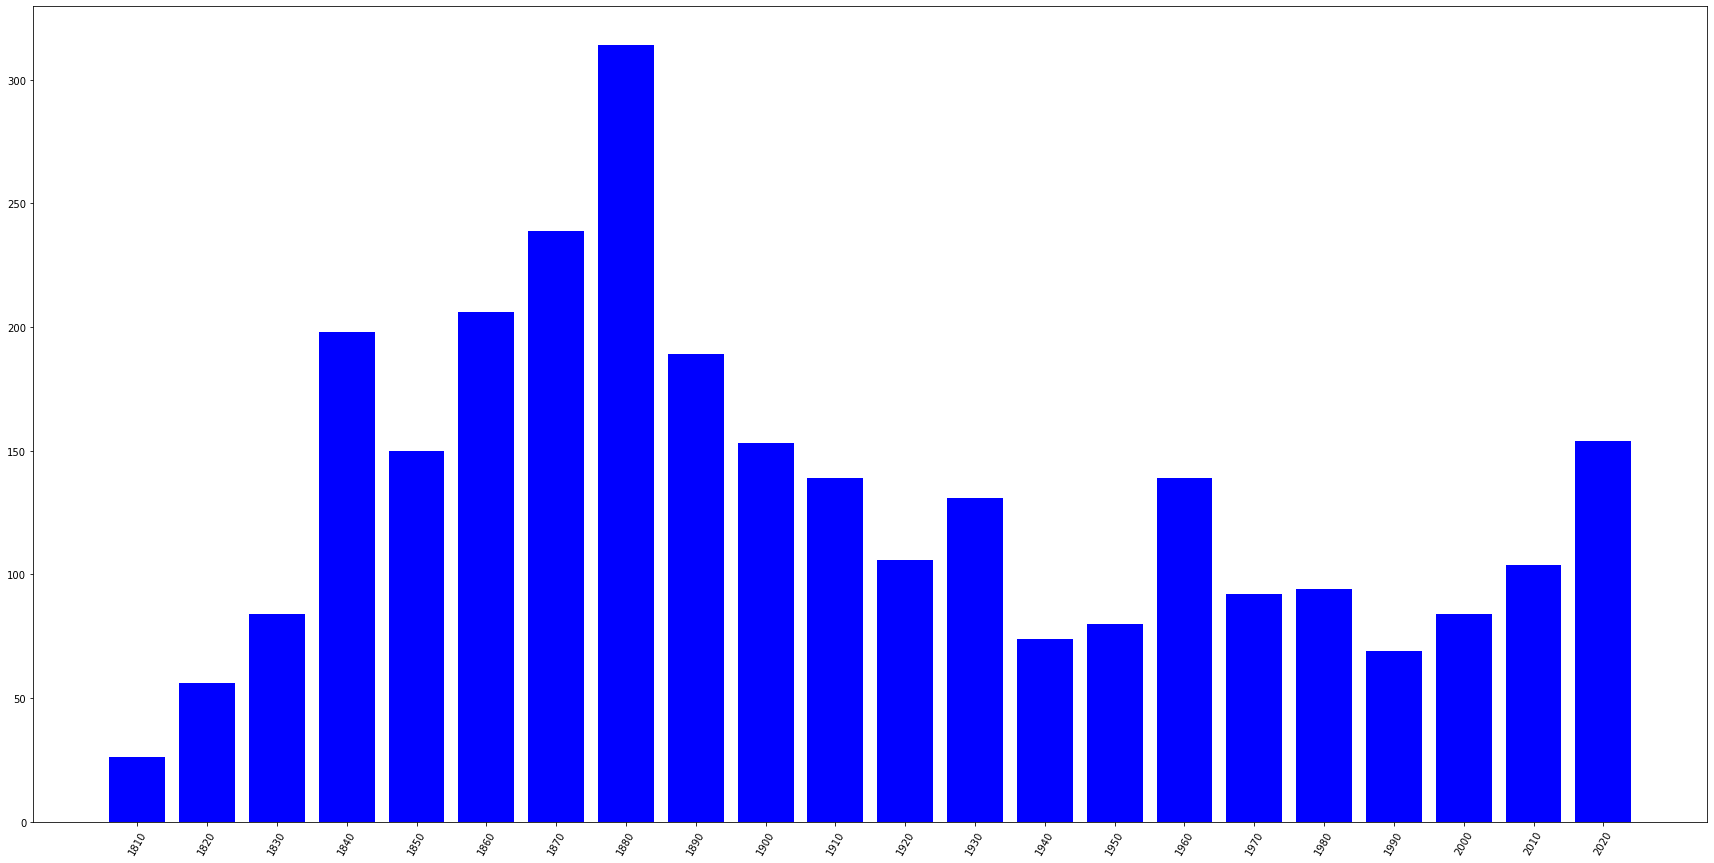
\includegraphics[width=15cm]{img/01_decades.png}
    \caption{Répartition du corpus dans le temps}
    \label{corpus_bar}
\end{figure}

La répartition dans le temps des romans de notre corpus est plutôt bonne, avec cependant la deuxième parie du XIX\ieme siècle qui comporte près de 40\% des romans. La décennie 1880 représente à elle seule près de 10\% des romans. Il faudra tenir compte de ces biais potentiels dans nos analyses, le risque étant de sur-représenter cette période dans les mesures statistiques. 

Le tableau \ref{Tab:statscorpus} décrit le corpus avec des statistiques simples. 

\begin{table}[ht]
\caption{Statistiques du corpus}
\centering
\bigskip
\begin{tabular}{lc}
    \hline
    Romans &  2953 \\
    Phrases &  14.982.817 \\
    Mots &  234.175.471 \\
    Moyenne de mots par roman & 79301 \\
    \hline
\end{tabular}
 \label{Tab:statscorpus}
\end{table}
\bigskip

L'un des biais principaux de ce corpus est qu'il rassemble les œuvres romanesques numérisées et disponibles sur internet. Cela implique nécessairement que ces textes ont été sélectionnés, publiés et conservés dans le temps, ce qui représente une partie infime de la production d'écrits. 

Pourtant, nous pensons que les ouvrages non-canoniques du corpus représentent un bon échantillon de ce qu'à pu être la production littéraire populaire, de par leur nombre - plus des 9/10 (cela dépend du critère que nous choisissons, nous verrons cela au prochain chapitre), mais aussi par la diversité des sous-genres représentés. La figure \ref{genres_corpus} montre les différents sous-genres du corpus, qui vont des romans policiers aux romans d'aventures, en passant par la science fiction. Il est important de noter que 2/3 des romans ont une étiquette de genre littéraire, ce qui représente selon nous un échantillon représentatif. Nous commenterons la répartition du canon dans le corpus en section \ref{notre_canon}.

\bigskip
\begin{figure}[!ht]
    \centering
    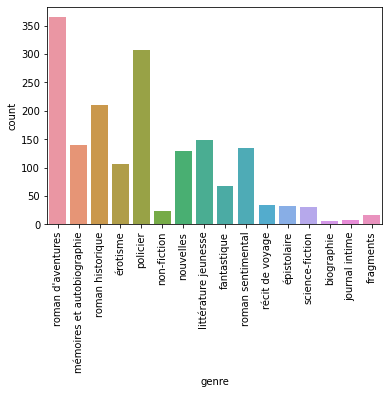
\includegraphics[width=15cm]{img/02_genres_corpus.png}
    \caption{Sous-genres littéraires du corpus}
    \label{genres_corpus}
\end{figure}



\chapter{Caractériser un canon littéraire}

\section{Méta-données : Enrichir le corpus}

Une des tâches principales du mémoire a été la construction d'un canon littéraire. Pour cela, nous entreprenons d'enrichir notre corpus avec les éléments de la réception actuelle des textes et des auteurs. Le canon littéraire n'est ni monolithique ni temporellement stable, le définir par des critères finis est en soi réducteur et néglige la complexité du phénomène. Mais nous allons essayer de nous focaliser sur des éléments déjà discutés et analysés par la critique littéraire et les études réalisées sur ce sujet. Un des aspects sur lequel nous allons nous concentrer est le rôle des institutions dans la formation du prestige littéraire. En premier lieu, tout le travail réalisé par Martine Jey et Laetitia Perret\footcites{jey_idee_2019} sur le rôle de l'institution scolaire dans la constitution de tels ensembles est prépondérant. Toutes deux ont montré que l'enseignement secondaire et supérieur avaient un impact énorme sur les processus de canonisation (dans la fabrication et surtout la conservation de ce canon) des auteurs et des textes. 


Travailler sur le canon littéraire à partir de la réception réalisée par les institutions scolaires nous paraît pertinent parce que cela s'inscrit dans une approche déjà éprouvée, bien qu'elle soit non exhaustive. En effet, d'autres facteurs entrent en jeu dans la constitution du canon, que ce soient des critères politiques, économiques ou sociologiques.

Il est important de noter que nous allons analyser la réception du canon littéraire par la réception actuelle, ce qui constitue aussi un élément discutable, mais la disponibilité des sources des méta-données (grâce à leur format numérique), nous a permis de recueillir énormément de données dans un temps réduit. 

Ainsi, nous avons établi un ensemble de critères non exhaustifs pour caractériser le canon littéraire que nous allons investiguer quantitativement.

\subsection{Le canon scolaire}

En premier lieu, nous nous sommes intéressés aux listes et au programmes des examens du secondaire, c'est à dire le brevet et le baccalauréat. Si l'on considère l'école républicaine comme le lieu de diffusion et de conservation du canon littéraire, alors il nous semble important de prendre en compte ce que l'on attend d'un élève lorsqu'il sort de l'enseignement obligatoire, c'est à dire ce qui constitue, pour les auteurs de ces listes, la culture littéraire minimale à la construction citoyenne. Le travail de Martine Jey, \enquote{La littérature au lycée : invention d’une discipline (1880-1925)}\footcites{jey_litterature_1998} décrit avec précision la construction d'une discipline, la littérature autour de textes garants d'une certaine langue et d'une certaine morale, qu'il faut diffuser pour éduquer les masses. Elle y analyse le processus d'intégration des œuvres dans le corpus scolaire qui est de fait un processus de canonisation. Au sein de l'enseignement scolaire et supérieur, les études littéraires produisent des formes distinctes de connaissances linguistiques\footnote{John Guillory, \enquote{Canon} in \cite{lentricchia_critical_2012},  p.43}. Il faudra donc récupérer des méta-données sur ces institutions qui construisent le canon littéraire.

%L'école fonctionne comme une institution sociale qui reproduit la structure stratifiée de l'ordre social.

\subsection{Le canon de l'enseignement du supérieur}

Dans un deuxième temps, nous nous sommes intéressés aux concours de l'enseignement du supérieur, qui incarnent le même rôle que précédemment mais avec un degré de prestige plus important. Nous avons récupéré les listes et les programmes de concours du supérieur (classes préparatoires littéraires et scientifiques du concours de l'ENS). Il s'agit d'évaluer et de sélectionner sur des connaissances littéraires, des candidats qui deviendront de futurs professeurs de collège. Michel P. Schmitt\footcites{schmitt_les_1993} a réalisé une démarche similaire en tenant des listes du nombre d'occurrences de citation d'auteurs dans les dissertations au CAPES interne. Sans passer par l'intérieur des copies, nous nous intéressons plutôt aux programmes des concours cités.

\subsection{Le canon des concours de l'agrégation}

Nous avons également récupéré les programmes des concours des agrégations de lettres modernes, plus haut concours de recrutement dans la fonction publique pour des professeurs. Il nous semblait significatif de constater quels étaient les auteurs et les textes sur lesquels on formait l'élite des professeurs de lettres de la République. Pour un panorama des épreuves de l'agrégation, les recherches de Martine Jey\footcites{jey_canon_2014}, d'André Chervel\footcites{chervel_histoire_1993} et de Yves Chevrel\footcites{chevrel_les_2003} ont été d'une grande aide.
Comme ces programmes ne comportaient pas beaucoup de romans, nous avons décidé d'agrandir la période de réception considérée. Pour cette méta-donnée précisément, nous remontons jusqu'en 1950.  

\subsection{Le canon des éditeurs}

Ensuite, nous nous sommes intéressés au monde de l'édition, qui est aussi un des acteurs majeurs dans le processus de canonisation des oeuvres. La thèse de Dragos Jipa\footcites{jipa_canonisation_2016} a bien montré, avec la collection des \enquote{Grands écrivains de France}, l'importance des logiques éditoriales dans la construction d'un consensus national autour d'un panthéon d'auteurs. 

Nous nous sommes intéressés à la collection de la Pléiade qui est l'exemple typique du rôle des éditeurs dans la canonisation d'auteurs. La publication des écrits d'un auteur en oeuvres complètes vient souvent parachever une carrière littéraire, souvent après la mort de l'auteur. Elle est un signe majeur dans la reconnaissance du-dit auteur en tant qu'appartenant au canon littéraire. C'est aussi une des portes privilégiées pour les éditeurs car elle permet de sacraliser de nouvelles têtes et d'en tirer profit par effet de levier. La collection de la Pléiade comporte finalement peu d'auteurs de romans, et consacre un auteur dans sa totalité. Malgré tout, nous récupérons tous les auteurs publiés dans la Pléiade.

% Quelle couverture XX vs XIX ème siècle ?
%+gné avant

Pour plus de finesse, nous prenons également l'édition Garnier-Flammarion et plus précisément la collection \enquote{littérature et civilisation}. Un des traits majeurs de cette collection est qu'elle présente les romans avec un appareil critique qui accompagne la lecture de l'ouvrage. Cet appareil critique n'est pas anodin et montre que l'ouvrage a une portée qui requiert explication. Le canon littéraire est rempli d'oeuvres qui valent la peine que l'on se penche sur elles et leur contextes. Cela nous intéresse parce que cette vision pédagogique du canon littéraire est très répandue et est même un des arguments au statu-quo littéraire en France et ailleurs\footcites{guillory_cultural_1998}.  

\subsection{Le canon de la critique}
Pour prendre un témoin de la critique littéraire, nous nous sommes intéressés aux prix littéraires. Ces derniers constituent la partie de notre canon la moins résistante au temps, car ils sont embourbés dans des dimensions économiques et politiques très fortes comme l'a résumé James F. English dans son livre sur la circulation de la valeur culturelle\footcites{english_economy_2009}. Malgré ces remarques, nous voulions mesurer son effet dans les pratiques littéraires. Ainsi nous avons récupéré les listes des prix littéraires les plus importants, du prix Goncourt au prix Femina. 

Enfin nous prenons en compte la recherche contemporaine, avec une canonicité à l'échelle de l'auteur et la revue littéraire en ligne \enquote{Fabula\footnote{https://www.fabula.org/}}. Cet aspect était déjà présent dans les méta-données du corpus Chapitres (voir en annexe \ref{chapitre}), et nous avons décidé de le conserver. 

\section{Notre canon}\label{notre_canon}

Ainsi construit avec plusieurs facteurs, notre canon littéraire se trouve moins discutable puisqu'il cherche à multiplier les entrées dans les différents acteurs du champ littéraire qui définissent, nourrissent et conservent le canon littéraire. 

Une grande partie de ces données, notamment celles du brevet et du baccalauréat ont été récupérées grâce à l'immense travail du collectif \textit{Le deuxième texte}\footnote{https://george2etexte.wordpress.com/} qui a mis en ligne ses données\footnote{https://www.data.gouv.fr/fr/organizations/le-deuxieme-texte/} en open source. D'autres ont été récupérées automatiquement à l'aide de scripts python sur les pages web de la collection Garnier-Flammarion et de la Pléiade, mais aussi à la main pour les auteurs présents dans le Lagarde et Michard (Bordas) du XIX\ieme siècle et du XX\ieme siècle.

Nous avons décidé d'établir une double approche quand à l'appartenance ou non au canon littéraire. La canonicité revient d'une part à la granularité du roman, et d'autre part à celle de l'auteur. 

Nous construisons ainsi deux canons littéraires, à l'échelle des auteurs et des textes. Nous mettons en annexes les listes détaillées de ces deux ensembles, avec en annexe \ref{canon_auteur} la liste des auteurs canoniques, et en annexe \ref{canon_roman} la liste des romans canoniques, triée par année de première parution. L'échelle de l'auteur agrandit énormément le cercle, puisque toutes les oeuvres d'un auteur canonique sont considérées comme canoniques. Si l'approche la plus intéressante nous paraissait la première à l'échelle de l'œuvre, nous avons conservé les deux qui méritaient tout autant des tests approfondis. 

Pour faire correspondre notre corpus au canon construit par nos soins, il a été décidé de réaliser un simple test d'appartenance, si le titre d'un roman appartient à au moins une liste, le roman en question est considéré comme canonique. Même chose pour l'auteur, s'il est présent dans une des listes établies, tous les textes de l'auteur sont considérés comme canoniques. Ainsi, le nombre des ouvrages du corpus qui sont dans notre canon s'élève à 264 éléments (moins de 1\% du corpus), tandis que le nombre des œuvres dont les auteurs sont dans notre canon est de 1156 romans, soit 39\%.

Nous avons pensé mettre en place un indice de canonicité, pour mieux représenter la réalité du monde littéraire, qui n'est pas d'une binarité sans conditions, entre canon et non canon. Un auteur est plus ou moins canonique, et Honoré de Balzac l'est plus qu'Anatole France par exemple. Mais nous manquions de temps et de données pour présenter une telle approche, et après des essais peu fructueux, nous conservons notre test d'appartenance binaire.

Pour bien vérifier la viabilité de ces approches, nous avons réalisé des statistiques descriptives pour voir comment notre canon se comportait dans le corpus. 

\bigskip
\begin{figure}[!ht]
    \centering
    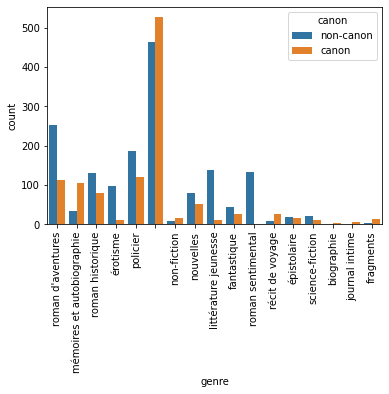
\includegraphics[width=15cm]{img/03_genres_corpus_canon.png}
    \caption{Répartition du canon dans les sous-genres du corpus}
    \label{genre_corpus_canon}
\end{figure}

On constate dans la figure \ref{genre_corpus_canon} une bonne répartition des oeuvres du canon des auteurs dans les sous-genres littéraires du corpus. Il faut souligner que les ouvrages canoniques sont de fait moins représentés que ceux canoniques, puisque le corpus en comporte seulement 39\%. La seule anomalie à constater est au sein des ouvrages non-étiquetés par un genre, où le canon est plus représenté que les non-canons. Mais la différence d'une cinquantaine d'ouvrages n'est pas énorme, et l'on ne peut pas conclure dans ce cas que le canon des romans n'est qu'un agrégat de sous-genres littéraires spécifiques.

\bigskip
\begin{figure}[!ht]
    \centering
    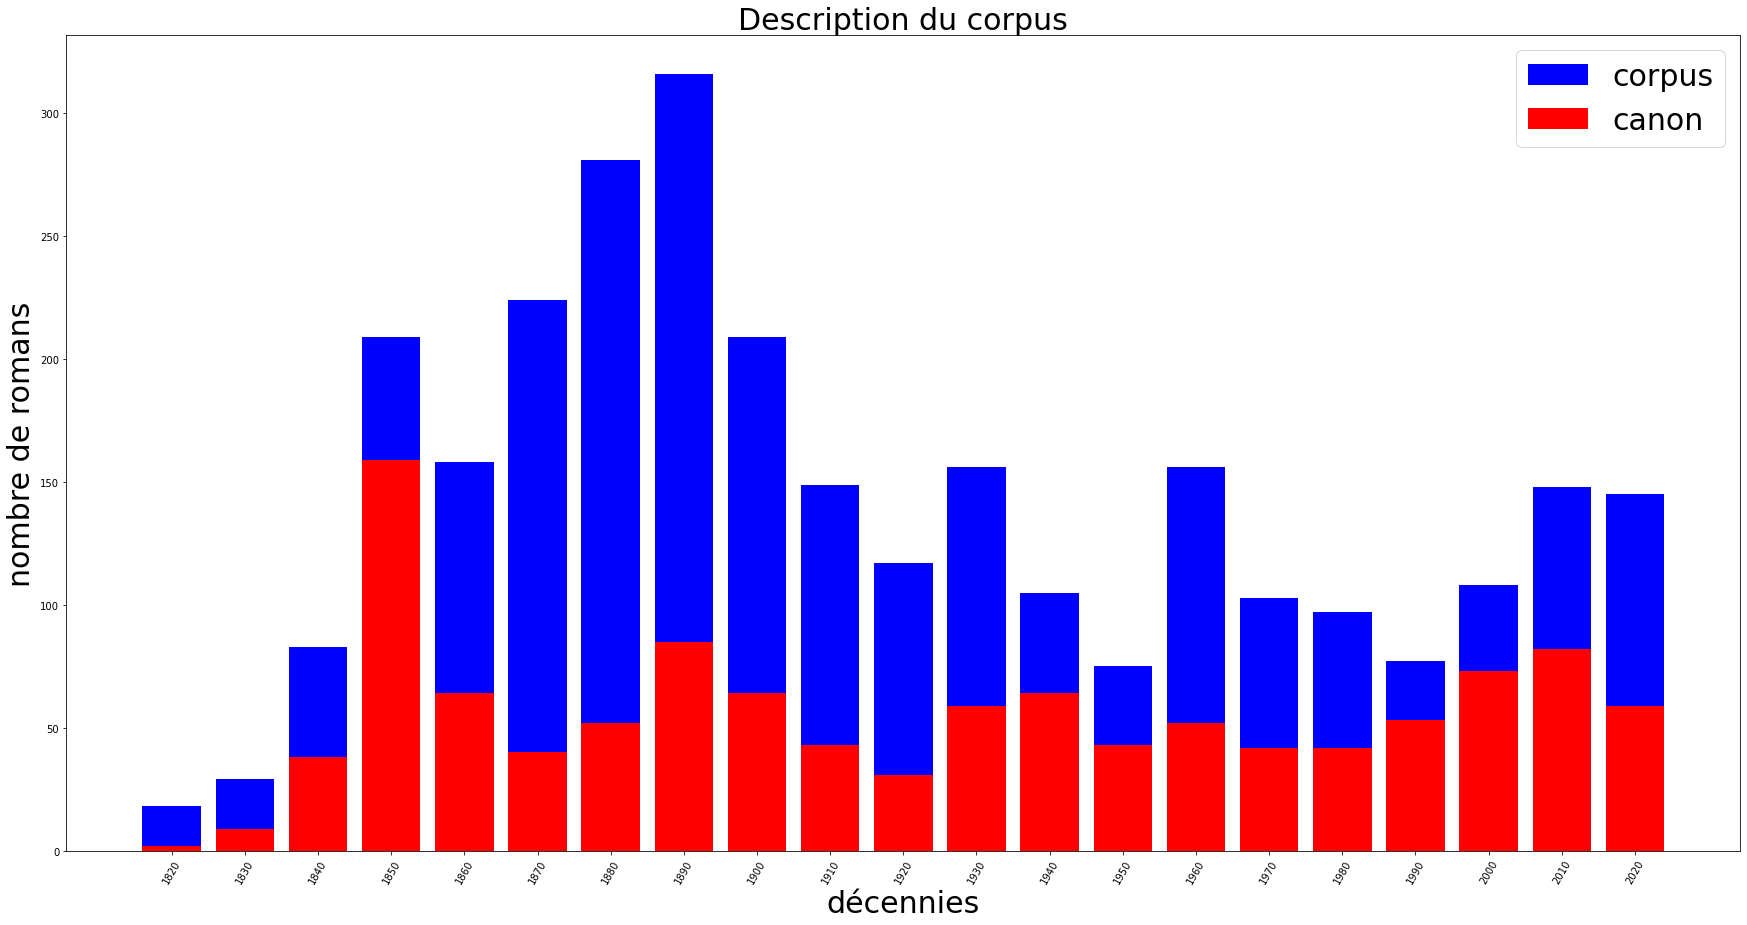
\includegraphics[width=15cm]{img/04_corpus_bar.png}
    \caption{Répartition du canon dans le temps}
    \label{corpus_bar_temps}
\end{figure}

La figure \ref{corpus_bar_temps} représente la présence de notre canon au fil de l'histoire littéraire. Il est assez bien réparti et suis l'évolution de la population du corpus. On remarque que la décennie de 1840 à 1850 comporte plus de canon que de non-canon, mais c'est la seule dans ce cas.

Ainsi, le genre littéraire ou la date de parution ne sont pas des facteurs définitifs pour expliquer la présence de romans ou d'auteurs dans le canon. Notre approche, qui est d'ouvrir les romans et de s'intéresser au contenu textuel de manière quantitative est justifié, dans le sens où le texte est un facteur qui pourrait contribuer à apporter des éléments de réponses. 


\chapter{Méthodes et outils}

Les méthodes du traitement automatique des langues sont d'une grande assistance. En plus de nous aider au pré-traitement et au nettoyage des textes, elles nous permettent de récupérer les caractéristiques textuelles sur lesquelles notre classification automatique se fonde. Nous présentons, dans les sections qui suivent, la méthode que nous mettons en place.

\section{Les données textuelles}

Nous voulons mettre au jour une esthétique canonique dans nos textes. On s'intéresse donc à des éléments formels, qui seraient des indices linguistiques issus de la filtration des textes jusqu'à la réception actuelle. Le phénomène que nous voulons modéliser est complexe, et pas évident puisque c'est un phénomène à réception, qui viendrait consacrer un texte ou un auteur après l'écriture de ses textes. Face à la complexité du phénomène que nous envisageons, nous avons voulu simplifier les caractéristiques textuelles retenues. En effet, le meilleur moyen de prendre en compte le contenu textuel de nos romans est de récupérer des informations sur les mots de ces derniers. Cette méthode a déjà été utilisée par des chercheurs déjà cités, notamment Ted Underwood dans son article \enquote{La longue durée du prestige littéraire}\footcites{underwood_longue_2016}.  Nous aurions pu prendre des éléments plus complexes, relatifs au style ou à la littérarité des ouvrages comme la longueur des phrases, l'avancée narrative ou les thèmes du récit. Mais la relation entre complexité du style, littérarité et prestige littéraire n'est pas si évidente que cela, et nous décidons d'une première approche \enquote{simple}, que l'on pourrait complexifier par la suite, si ces premières recherches se trouvaient fructueuses.

Ainsi nous décidons de transformer nos ouvrages en \textit{sac-de-mots}. Les textes sont ainsi décomposés en des listes de mots qui indexent leur fréquence relative (le nombre de fois où l'unité apparaît, divisé par la longueur totale du texte). Chaque unité est traitée comme une caractéristique des textes dans lesquels elle apparaît - une sorte de trait d'identification - et le texte devient un vecteur de ces traits. 

Nous décidons de limiter notre sac de mots au 1000 uni-grammes les plus fréquents récupérés dans un échantillon de 200 textes tirés au hasard dans le corpus.  Deux raisons à cela, une première pratique, puisque la prise en compte de tous les mots du corpus aurait nécessairement amené à des coûts computationnels très importants, car les matrices résultantes auraient été très éparses, avec beaucoup de fréquences d'apparitions nulles ou proches de zéro. La seconde raison réside dans la nature des mots que nous récupérons. Comme ce sont les mots les plus fréquents du corpus, la plupart sont des déterminants, prépositions et autres \textit{mots-outils}. Ces derniers relèvent plus d'une écriture inconsciente et automatique des auteurs qu'à des mots moins fréquents relatifs au contenu et aux thèmes du textes. Il ne nous semble pas que les mots de nature thématique jouent un rôle dans la spécificité des textes à être canoniques ou non. Cela nous permet également de ne pas prendre en compte une grande majorité des noms communs ou des noms propres, qui ne nous intéressent pas à cette échelle.

Ces \textit{mots-outils} sont au coeur de la stylométrie, notamment dans les attributions d'auteur\footcites{burrows_delta_2002}, et dans l'étude des idiolectes\footcites{seminck_evolution_2022}, c'est à dire de la signature textuelle d'un écrivain. Ces méthodes ont produit de très bons résultats, allant de Hildegarde de Bingen\footcites{kestemont_function_2014}, à Shakespeare\footcites{plechac_relative_2021} ou Molière\footcites{cafiero_why_2019} et Racine\footcites{cafiero2021psyche}. Si le problème auquel nous faisons face n'est pas de même nature, nous pensons que ces techniques sont pertinentes pour traiter notre problème. En effet, s'il y a bien une manière particulière de faire littérature selon les institutions qui forment le canon littéraire, alors nous devrions retrouver les marqueurs inconscients de cette sélection. 

Pour quantifier les fréquences d'apparition de mots, on réduit les unités lexicales sujettes à flexion (les verbes, les substantifs, les adjectifs) à leur unité lexicale commune. On appelle ce processus \textit{lemmatisation}. Pour ce traitement, nous utilisons la librairie Spacy. Elle nous permet de tokeniser, lemmatiser et de nettoyer les romans en contrôlant l'étiquetage morphosyntaxique des tokens. La figure \ref{work_flow} représente la chaîne de traitement de la récupération des données textuelles.

\bigskip
\begin{figure}[!ht]
    \centering
    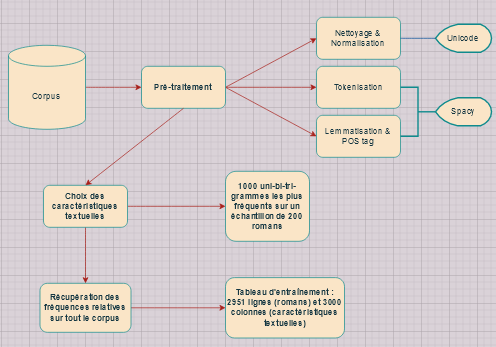
\includegraphics[width=15cm]{img/05_work_flow.png}
    \caption{Récupération des données textuelles : Flux de travail}
    \label{work_flow}
\end{figure}

Des recherches récentes en classification de textes littéraires ont montré que la prise en compte des contextes d'un mot pouvait avoir des impacts important sur les résultats d'une classification\footcites{van_cranenburgh_identifying_2015}. Ainsi, nous décidons de prendre en compte, en plus des uni-grammes, des bi-grammes et des tri-grammes de lemmes. Ces derniers sont agrégés par la concaténation de deux ou trois lemmes. Nous procédons de la même manière que pour les uni-grammes, en prenant les 1000 éléments les plus fréquents pour chaque type.

Finalement, nous obtenons un grand tableau de données, avec en colonnes les trois mille caractéristiques textuelles que l'on vient de définir, et en lignes chaque roman de notre corpus. Le tableau est rempli avec les fréquences relatives pour chaque caractéristique.  

\section{Outils de programmation}

Nous fondons notre travail sur le langage de programmation Python et les librairies construites au-dessus. Pour l'analyse des données et leur manipulation nous utilisons Pandas\footnote{https://pandas.pydata.org/} et Numpy\footnote{https://numpy.org/}. Pour le traitement du texte à proprement dit, nous employons la librairie Spacy\footnote{https://spacy.io/}. Cette dernière est très performante pour une analyse sur de grandes quantités de données et couvre tous les traitements d'une chaîne de TAL classique. Cette librairie est un peu moins performante pour le français des textes littéraires, parce qu'elle a été entraînée sur des contenus de presse récente. D'autres librairies proposent des modèles un peu plus performants, comme la librairie Stanza\footnote{https://github.com/stanfordnlp/stanza} ou Pie-Extended\footnote{https://github.com/hipster-philology/nlp-pie-taggers}. Pour autant, après des tests de ces différentes librairies, Spacy se montrait la plus efficace en terme de temps d'exécution, avec un nombre d'erreurs plus important que les deux autres mais relativement réduit dans l'ensemble. Avec nos moyens informatiques limités, nous avons privilégié cette librairie pour parser nos 3000 romans. Cette dernière a aussi l'avantage d'être très bien documentée et comporte plusieurs modèles de langages pour le français. Au vu des performances des différents modèles, nous prenons la décision d'utiliser le modèle fr\_core\_news\_lg qui a un très bon rapport d'utilisation de ressources temporelles et matérielles entre exécution et performance. Nous utilisons aussi Scikitlearn\footnote{https://scikit-learn.org/stable/index.html}, qui donne des outils efficaces pour l'analyse prédictive de données. Scikitlearn est assez simple à utiliser et implémente des algorithmes d'apprentissage machine au niveau de l'état de l'art.

\section{Modélisation statistique}

Nous voulons observer si des différences statistiques majeures existent entre nos deux sous-corpus, celui canonique et celui non-canonique. Nous faisons appel au champ de recherches de l'apprentissage machine. L'objectif de la modélisation statistique est de tirer des généralisations sur de grands jeux de données. Un exemple explicite est la régression linéaire, qui cherche à établir une relation entre des variables diverses. 

L'apprentissage machine fait référence à toute une série d'algorithmes statistiques qui traitent chaque texte comme un amalgame de certaines caractéristiques quantifiables. Cette approche part du principe que l'on peut quantifier leur répartition dans les textes de manière à identifier les différences entre ces derniers, afin de classifier ou prédire la catégorie à laquelle un texte est susceptible d'appartenir. 

%L'intérêt de l'apprentissage automatique est justement de modéliser des pratiques de catégorisation qui n'ont pas de définition et qui peuvent être déduites uniquement d'exemples. Nous ne savons peut-être pas comment décrire un spam, même si nous le reconnaissons dans notre boîte mail. Un filtre anti-spam commence donc par un apprentissage composé de messages que les lecteurs ont ou n'ont pas marqué comme spam. Un algorithme apprend à modéliser le spam en utilisant tous les détails textuels qui, en pratique, distinguent ces groupes de groupes de messages.

La classification automatique de textes est un problème très étudié en statistiques. Plusieurs estimateurs sont au niveau de l'état de l'art : des modèles linéaires, comme le naïve bayes ou la classification ridge. Une famille de modèle retient particulièrement notre attention parce qu'elle obtient de bons résultats pour la classification de textes littéraires: les Machines à Vecteur de Support (SVM)\footcites{yu_evaluation_2008}. Les SVM ont pour but de trouver les plans qui séparent les points de données avec les marges maximales entre les frontières de décision. Ils traitent les caractéristiques comme des coordonnées dans un espace cartésien à haute dimension et tentent de tracer une ligne qui divise au mieux les caractéristiques uniques d'une classe\footnote{Pour de plus amples informations sur les SVM, voir l'article fondateur de Vladimir Vapnik dans \cites{cortes_support-vector_1995}}. Pour l'estimateur SVM, un texte n'est qu'une combinaison de caractéristiques qui tendent à apparaître plus souvent dans une classe de textes que dans une autre. Le modèle assigne des coefficients à chaque mot pour estimer la probabilité que le roman soit canonique. 

Les SVM ont l'avantage de réduire le risque de sur-apprentissage. Ce dernier se caractérise lorsqu'un modèle statistique se spécialise trop sur ses données d'entraînement, ce qui réduit sa performance de généralisation. Nous utilisons dans ce mémoire la famille de SVM développé par l'équipe scikit-learn\footcites{scikit-learn_2011} depuis 2011.

Nous avons affaire à une approche très connue en apprentissage machine : l'apprentissage supervisé. Ce dernier est assez simple à comprendre, puisqu'il associe un ensemble de données avec une certaine classe labellisée. Un modèle statistique est évalué sur sa capacité à faires des inférences entre les particularités des données et une certaine classe. Les classes de nos romans correspondent aux méta-données récupérées, c'est à dire si le roman en question appartient ou non au canon littéraire.

\subsection{Implémentation de l'apprentissage machine}

Nous mettons en place les bases de l'apprentissage machine. Le jeu de données est séparée en deux échantillons. 

\begin{itemize}
    \item Un premier sur lequel nous entraînons le modèle statistique, c'est à dire que nous lui donnons le label associé pour chaque roman.
    \item Un autre sur lequel nous évaluons ses performances de prédictions sur des données qu'il n'a jamais vu. 
\end{itemize} 

Nous mesurons ainsi la capacité du modèle à généraliser.

Nous voudrions que la taille de l'échantillon du corpus d'entraînement soit la plus large possible, pour donner toutes ses chances au modèle. Pour autant, il est important de garder une taille conséquente pour l'échantillon de test afin de mesurer à quel point le modèle est capable de réaliser de bonnes prédictions sur un grand nombre de données. Nous fixons la taille de l'échantillon test à 20\% du total. 

Nous implémentons grâce à Scikitlearn un pipeline avec un pré-traitement des données, un StandardScaler et un estimateur, le SVM. Ce pré-traitement permet de normaliser nos données. La normalisation d'un ensemble de données est une exigence commune à de nombreux estimateurs d'apprentissage automatique : ils peuvent mal se comporter si la distribution statistique ne ressemble pas à des données distribuées sous forme d'une loi normale. Nous avons implémenté le SVM du logiciel SuperStyl\footcites{Camps_SUPERvised_STYLometry_SuperStyl_2021}, de Jean-Baptiste Camps, puis nous avons codé un algorithme mieux adapté à notre approche, avec des estimateurs plus performants et une méthode spécifique pour une classification binaire.\footnote{Voir en annexe \ref{code} le lien du github avec le code du mémoire} 

Nous contrôlons la robustesse de nos résultats par une validation croisée en cinq parties. Cette validation est une procédure qui permet d'éviter le sur-apprentissage et de garantir la fiabilité de nos modèles. Elle sépare l'ensemble du jeu de données en cinq parties, et réalise cinq entraînements distincts en prenant à chaque fois quatre parties pour l'entraînement et une pour s'évaluer. La moyenne de l'efficacité du modèle sur ces cinq entraînements est ainsi un score beaucoup plus robuste et fiable. 

\subsection{Métriques d'évaluation du modèle}

Nous évaluons notre modèle grâce à des métriques d'évaluation de la performance : l'efficacité, la précision, le rappel et un f1-score.

Pour comprendre ces métriques, il faut se familiariser avec les notions de vrai-positif (TP), vrai-négatif (TN), faux-positif (FP) et faux-négatif (FN). Dans notre cas, un TP est un roman considéré comme canonique par nos méta-données et prédit comme tel. Un TN est un roman non-canonique prédit comme non-canonique. Un FP est un roman non-canonique prédit comme canonique. Un FN est un roman canonique prédit comme non canonique. Une prédiction sans erreur équivaut donc à minimiser les mauvaises attributions, c'est à dire minimiser FP et FN. 

L'efficacité est la métrique la plus simple à comprendre, puisque c'est le pourcentage d'éléments prédits correctement par le modèle. 

\begin{equation}
Efficacite = \frac{TP + TN}{TP + TN + FP + FP}.
\end{equation}


\bigskip
\begin{figure}[!ht]
    \centering
    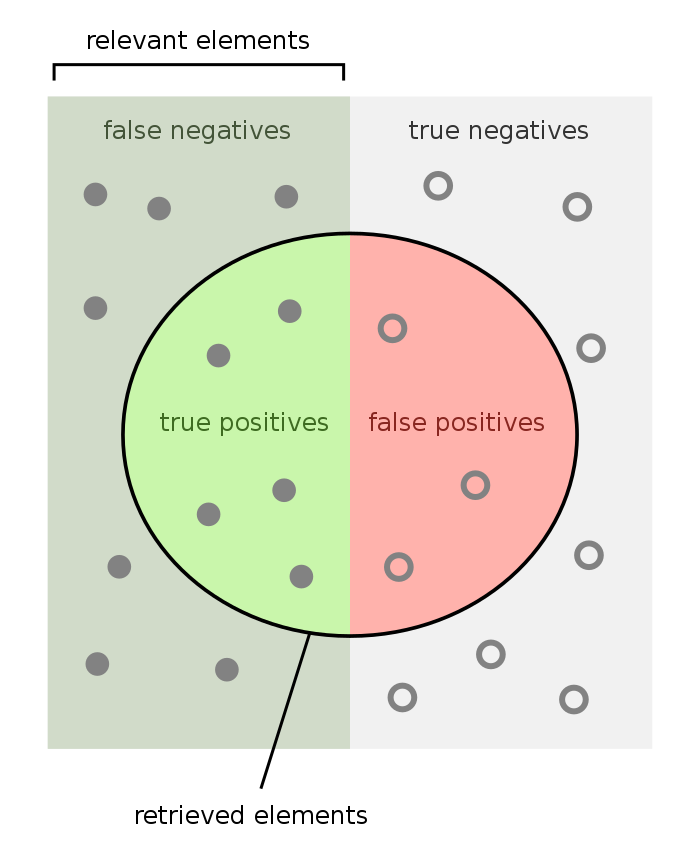
\includegraphics[width=10cm]{img/06_precision_recall.png}
    \caption[Précision et rappel 1/2]{Précision et rappel 1/2\footnotemark}
    \label{modelevaluation}
\end{figure}


Comme on peut le voir sur la figure \ref{modelevaluation}, la précision est la fraction d'éléments pertinents parmi les éléments extraits. Autrement dit, la précision est définie par : 

\begin{equation}
Precision = \frac{TP}{TP + FP}.
\end{equation}
 

Le rappel est la fraction d'éléments pertinents qui ont été extraits. Autrement dit, le rappel est définie par :
\begin{equation}
Rappel = \frac{TP}{TP + FN}.
\end{equation} 
\footnotetext{\textit{ Source : }$https://en.wikipedia.org/wiki/Precision\_and\_recall$}

\bigskip
\begin{figure}[!ht]
    \centering
    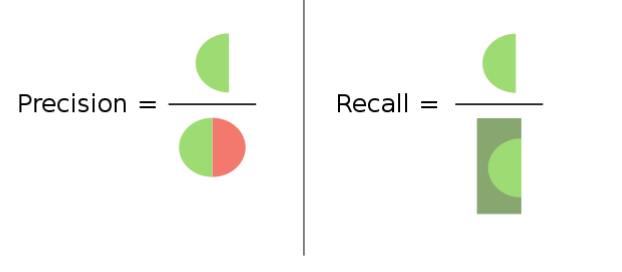
\includegraphics[width=10cm]{img/07_preci_recall.png}
    \caption[Précision et rappel 2/2]{Précision et rappel 2/2\footnotemark}
    \label{preci_recall}
\end{figure}

\footnotetext{\textit{ Source : }$https://en.wikipedia.org/wiki/Precision\_and\_recall$}

Le score F1 peut être interprété comme une moyenne harmonique de la précision et du rappel, où un score F1 atteint sa meilleure valeur à 1 et son pire score à 0. La formule pour le score F1 est la suivante : F1 = 2 * (précision * rappel) / (précision + rappel)

Il faut être attentif à ces trois métriques pour s'assurer de la viabilité du modèle et de sa performance. En effet, même lorsque l'efficacité du modèle est très bonne, les autres mesures peuvent, par exemple dans le cadre d'un jeu de données peu équilibré, montrer les limites du modèle en donnant des scores très bas.


Ainsi, nos expérimentations se fondent sur trois piliers principaux. Un corpus d'étude, un canon construit par nos soins et les méthodes quantitatives. A partir de cela, nous proposons de modéliser la notion de canon littéraire pour poser un diagnostique quantitatif de la filtration du contenu littéraire au cours du temps.
\part{Résultats et discussions}

\chapter{Une esthétique canonique multi-échelle}

Dans ce chapitre, nous présentons les résultats de nos différentes approches. Les hypothèses du mémoire semblent se vérifier statistiquement, et nous évaluons leur solidité statistique avec différentes métriques et différentes approches. 

\section{A l'échelle du roman}

Le modèle parvient à 75.3\% d'efficacité en validation croisée à l'échelle du roman. Dans notre cas de classification binaire, cela veut dire que la prédiction de la canonicité se révèle être bonne pour trois textes sur quatre. Il est admis que les résultats d'un modèle statistique sont fiables lorsque ses performances atteignent entre 75\% et 80\% d'efficacité, si les autres métriques du modèle convergent vers une stabilité autour de ces valeurs.

	\begin{table}[ht]
		\centering % Centre the table on the slide
		\begin{tabular}{l c c c c c}
			\toprule
    			 & precision & recall & f1-score & support & accuracy \\
			\toprule
			canon & 0.746 & 0.598 & 0.662 & 52 \\
			\midrule
			non-canon & 0.754 & 0.858 & 0.806 & 76\\
			\midrule
			full dataset & & & & 128 &\textbf{0.753} \\
			\midrule
			macro-average & 0.752 & 0.728 & 0.732 & 128\\
			\midrule
			weighted average & 0.751 & 0.751 & 0.746 & 128\\

			\bottomrule
		\end{tabular}
	\caption{Résultats de l'évaluation du modèle en validation croisée}
	\end{table} 
% see https://datascience.stackexchange.com/questions/86537/scikit-learn-classification-reports-f1-accuracy
Le modèle prédit mieux les ouvrages non-canoniques que les autres, mais le score de précision est plutôt bon (0.746). C'est le rappel (recall) qui pose des problèmes à notre modèle, c'est à dire que lorsqu'il prédit le label canonique il se trompe rarement, mais il n'arrive pas à le prédire dans un grand nombre de cas. Nous voyons là des signes du déséquilibre encore présent dans nos échantillons d'entraînement. 

Pour renforcer les résultats, nous entreprenons une démarche aléatoire pour nous assurer que le modèle statistique détecte bien des différences textuelles associées à nos méta-données plutôt que d'arriver artificiellement à séparer les deux classes. Cette approche aléatoire se réalise assez facilement, en désignant une classe canon ou non canon aléatoirement pour tous nos romans. Les résultats oscillent entre 45\% et 55\% d'efficacité, ce qui montre bien que le SVM n'arrive pas à séparer artificiellement nos deux classes sans raisons textuelles latentes. Ainsi, il se passe véritablement quelque chose dans les ouvrages canoniques. Nous désignons par dialecte canonique ce résultat, dont nous discuterons dans la suite du mémoire. 

\bigskip
\begin{figure}[!ht]
    \centering
    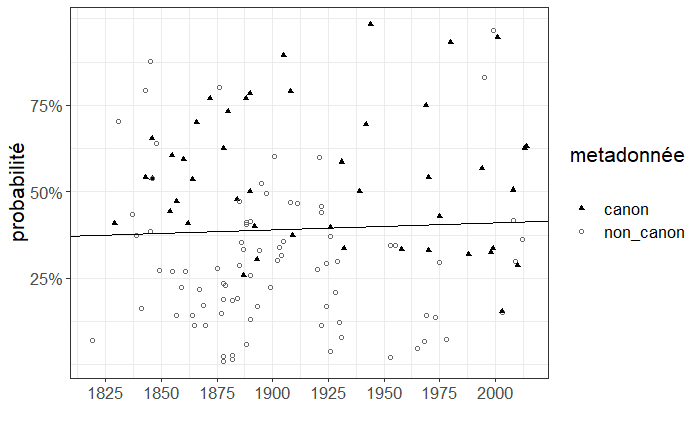
\includegraphics[width=15cm]{img/08_main_vis_svm.png}
    \caption{Probabilité prédite d'appartenir au canon littéraire, canon des romans}
    \label{svm_novel}
\end{figure}

Dans la figure \ref{svm_novel}\footnote{Nous reproduisons ici la visualisation de Ted Undewood dans son livre \cite{underwood_distant_2019}, page 80, voir \cite{underwood_tedunderwoodhorizon_2018} pour le code} nous projetons la probabilité prédite de chaque roman à appartenir au canon littéraire. Tous ces romans proviennent de l'échantillon de test, sur lequel on évalue la performance de généralisation du modèle. Les triangles représentent les romans classés comme canoniques et les cercles ceux non-canoniques. Le SVM arrive assez bien à détecter les deux classes, peu de romans canoniques sont classés non-canoniques, à l'exception de la fin du XX\ieme siècle, où le modèle fait quelques erreurs. La droite correspond à une régression linéaire de l'ensemble des probabilités canoniques assignées à chaque roman par notre modèle. Nous constatons ainsi une légère hausse de cette probabilité au cours du temps et nous commenterons ce résultat qui se renforce à l'échelle des auteurs.


\section{A l'échelle de l'auteur}

Le modèle atteint 90.4\% d'efficacité en validation croisée à l'échelle de l'auteur. Les résultats sont ainsi nettement meilleurs qu'à l'échelle des romans. 
	\begin{table}[ht]
		\centering % Centre the table on the slide
		\begin{tabular}{l c c c c c}
			\toprule
    			 & precision & recall & f1-score & support & accuracy \\
			\toprule
			canon & 0.866 & 0.888 & 0.878 & 231 \\
			\midrule
			non-canon & 0.928 & 0.911 & 0.921 & 361 \\
			\midrule
			full dataset & & & & 592 & \textbf{0.904}\\
			\midrule
			macro-average & 0.898 & 0.902 & 0.898 & 592 \\
			\midrule
			weighted average & 0.904 & 0.904 & 0.904 & 592 \\

			\bottomrule
		\end{tabular}
	\caption{Résultats de l'évaluation du modèle en validation croisée}
	\end{table} 

\bigskip
\begin{figure}[!ht]
    \centering
    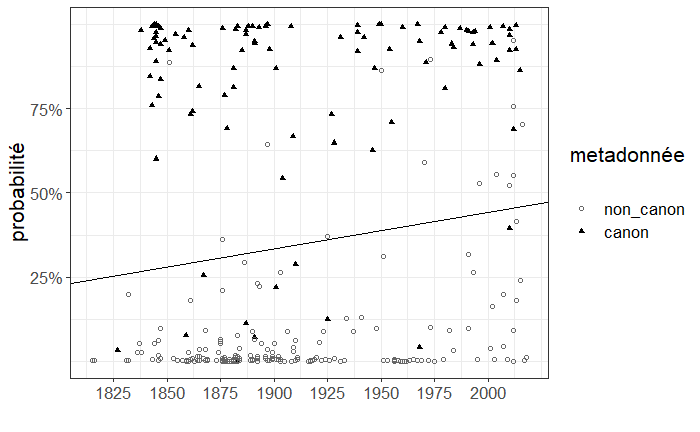
\includegraphics[width=15cm]{img/09_fabula_visual_svm.png}
    \caption{Probabilité prédite d'appartenir au canon littéraire, canon des auteurs}
    \label{svm_author}
\end{figure}


Dans la figure \ref{svm_author} nous projetons de la même manière la probabilité prédite de chaque roman à appartenir au canon littéraire, avec les méta-données canoniques à l'échelle de l'auteur. On remarque que le SVM est bien meilleur à cette échelle, c'est à dire bien plus confiant dans ses prédictions qu'à l'échelle des romans. Les deux groupes sont très distincts sur la figure \ref{svm_author}, et les erreurs sont moins nombreuses.   


Au regard de ces résultats, nous nous sommes demandés si le modèle ne détectait pas des indices linguistiques d'un groupe d'auteurs. 

Nous voulions savoir si le modèle ne reconnaissait pas l'idiolecte des auteurs canoniques sur lequel il s'était entraîné présents dans les œuvres de l'échantillon test. Si cela se vérifiait, notre modèle serait capable de réaliser des attributions d'auteurs et non de détecter un dialecte canonique. 

Ainsi nous avons entrepris de créer des jeux de données ne comportant qu'un roman par auteur pour exclure la probabilité que le modèle ne reconnaisse les ouvrages canoniques par la signature textuelle de leur auteur. Les résultats de cette démarche gardent une très bonne stabilité, c'est à dire que le modèle détecte bien quelque chose sans relation explicite avec les auteurs. 

Une des raisons qui pourraient expliquer la différence dans les performances entre les deux échelles de canonicité serait la taille de l'échantillon sur lequel le modèle est entraîné. En effet un défaut du SVM est de favoriser la classe la plus importante du jeu de données. Notre canon littéraire, à l'échelle du roman, n'est constitué que de 264 éléments, et même avec des procédures d'apprentissage non-équilibrées, il faut faire attention à la répartition des classes dans le jeu de donnée de l'échantillon d'entraînement. Ainsi, nous avons mis en place un ratio de répartition d'au moins 35\% de romans canoniques et 65\% de non canoniques au maximum. Le problème est que lorsque l'on travaille avec l'indice de canonicité à l'échelle des romans, la taille de l'échantillon de travail est moins important que celui à l'échelle des auteurs, de l'ordre de 800 éléments pour l'échelle de canonicité des romans et tout le corpus (3000 romans) à l'échelle des auteurs. De nombreux auteurs considérés comme canoniques ont beaucoup écrit d'ouvrages, cela explique la grande différence entre nos deux approches. Avec ce ratio et des procédures implémentées grâce à la librairie python imblearn\footnote{https://imbalanced-learn.org/stable/index.html}, le modèle fait des progrès de l'ordre de 5\% d'efficacité.

La régression linéaire projetée sur le graphe témoigne d'une tendance globale détectée par notre modèle. La probabilité d'appartenir au canon littéraire augmente avec le temps. Techniquement, cette hausse est une erreur. Les romans ne sont pas plus susceptibles d'appartenir au canon littéraire parce qu'ils sont publiés plus tard. Mais cela veut dire que le modèle échoue à produire des critères valides pour deux siècles de production littéraire. Les livres publiés plus tard comportent plus de signes linguistiques associés au canon littéraire. On remarque qu'une majorité des erreurs du modèle se trouvent entre les années 1975 jusqu'à nos jours. Des romans non canoniques (dont l'auteur n'est pas considéré comme canonique), obtiennent un bon score de canonicité. Le modèle perd en assurance et de nombreux romans se trouvent dans un entre-deux. On pourrait expliquer cela par une usure de la norme canonique, qui n'est plus aussi facile à discerner depuis les années 1975, malgré une distinction très forte durant 150 ans. 

En plus de ces hypothèses, on pourrait invoquer les limites de l'expérience pour expliquer cette tendance. En effet, on remarque que beaucoup de données tests se situent dans la deuxième partie du XIX\ieme siècle, où par ailleurs le modèle est très performant. C'est peut-être un biais du corpus que nous avons là, puisque cette période est proportionnellement très représentée dans notre corpus, comme on peut le constater en figure \ref{corpus_bar}. Le modèle a plus de données d'entraînement sur cette période, donc il se spécialise dessus. Pour autant, ce sur-apprentissage ne semble pas rédhibitoire puisque les données sont très bonnes sur les autres périodes aussi. Cela témoigne plutôt de la stabilité de la norme esthétique, puisque notre modèle repose en partie sur un léger sur-apprentissage des données plus nombreuses de la deuxième partie du XIX\ieme siècle, mais est capable de généraliser sur la longue durée.


\chapter{Discussions}

\section{Étude des cas limites}

L'étude des erreurs les plus importantes de nos modèles peut dire beaucoup de la manière dont ils se comportent. 

\begin{figure}[!ht]
    \centering
    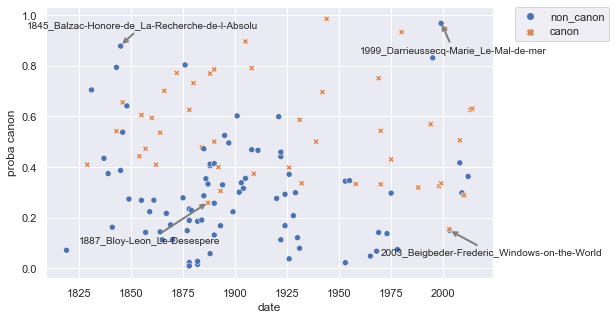
\includegraphics[width=15cm]{img/10_outliers_main_results.png}
    \caption{Cas limites du modèle entraîné à l'échelle des romans}
    \label{outlier_novel}
\end{figure}

La figure \ref{outlier_novel} met en avant quatre erreurs du modèle. Nous rappelons qu'à cette échelle le modèle performe à 75\% d'efficacité, donc les erreurs sont assez nombreuses. La canonicité prédite du roman de Balzac \textit{La recherche de l'absolu} est très importante, avec près de 90\% de probabilité. Pourtant, ce roman ne fait pas partie de notre canon littéraire. Ce roman de Balzac est classé dans les Études philosophiques de La Comédie humaine. Pour notre modèle, ce roman remplit tous les critères linguistiques relatifs au canon littéraire. Il en va de même pour le roman de Marie Darrieussecq, \textit{Le mal de mer}, qui pourtant est publié 150 années plus tard. Ce dernier n'est pas particulièrement resté dans les mémoires, du moins il n'est pas rentré dans un processus de canonisation. Pourtant, notre modèle le détecte comme tel. Cela peut re-légitimer cette œuvre, qui, au moins dans son contenu linguistique, fait aussi bien que les grands classiques de la littérature française. On constate d'autres erreurs du modèle dans le sens inverse. Des textes appartenant à notre canon littéraire ne sont pas bien notés par le modèle statistique. Par exemple, \textit{Windows on the world}, de Frédéric Beigbeder, fait parti de notre canon puisqu'il a gagné le prix Interallié en 2003. Ce roman relate les dernières minutes des victimes des attaques du World Trade Center le 11 septembre 2001. On constate ici les limites de nos méta-données, puisque le roman en question a pour vocation de raconter une histoire qui puisse toucher beaucoup de gens, en les amenant sur un sujet qui a bouleversé la société, plus que celle de rentrer dans le canon littéraire. \textit{Le désespéré}, est le premier roman de Léon Bloy, publié en 1887. Ce roman est canonique parce qu'il a été republié dans la collection \textit{Littérature Classique} de Garnier Flammarion en 2010. Il n'est pas aisé de comprendre pourquoi ce roman ne correspond pas à l'esthétique canonique perçue par notre modèle. Pour autant, la singularité de cette œuvre a été soulignée par Pierre Glaudes dans l'appareil critique de la réédition : \enquote{\textit{Le désespéré} est surtout un aérolithe littéraire, écrit dans une langue barbelée de mots rares, étrangement mystique, une œuvre d'une surprenante modernité}. Il semble que notre modèle donne raison à Pierre Glaudes, le roman sort des conventions et de l'esthétique du canon littéraire. 


A l'échelle des auteurs, le modèle est bien plus performant, mais quelques erreurs restent à noter comme on peut le voir en figure \ref{outlier_author}. 
\begin{figure}[!ht]
    \centering
    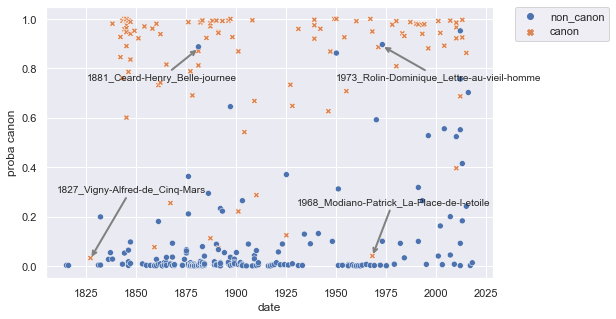
\includegraphics[width=15cm]{img/11_outliers_fabula_results.png}
    \caption{Cas limites du modèle entraîné à l'échelle des auteurs}
    \label{outlier_author}
\end{figure}

On a par exemple la \textit{Belle journée} d'Henry Céard qui est très bien noté par le modèle. Paru en 1881, ce roman est une ré-interprétation de \textit{Madame Bovary}, en forme d'hommage à Flaubert, mort un an auparavant. Henry Céard est un disciple de Flaubert et de Zola, son style se rapproche de ces derniers, même si l'histoire littéraire n'a pas retenu cet auteur. On peut donc expliquer cette erreur par la démarche même du roman qui est une imitation du style et du thème du roman de Flaubert. De la même manière, le livre de Dominique Rolin \textit{Lettre au vieil homme}, publié en 1973 est perçu comme canonique par le modèle, alors que l'écrivaine n'est pas retenue dans notre canon littéraire.

Au contraire, le roman \textit{Cinq mars}, d'Alfred de Vigny, est dans notre canon mais n'est pas admis comme tel par le modèle. Ce roman est considéré comme le premier roman historique, et l'on peut émettre l'hypothèse que c'est en cela qu'il se démarque de la manière commune de faire des romans pour notre modèle statistique. Enfin, le roman de Patrick Modiano \textit{La place de l'étoile}, publié en en 1968 aux éditions Gallimard est lui aussi très mal noté par le modèle. Le registre parodique du roman semble expliquer le fait qu'il n'ait pas sa place dans le canon littéraire perçu par le modèle.

%A l'échelle d'un auteur ? Flaubert ou Maupassant par ex ?


\section{Caractéristiques discriminantes du modèle statistique}

Il faudrait maintenant comprendre comment nos modèles statistiques sont capables de prédire la canonicité. Un des intérêts de l'apprentissage machine est d'ailleurs la possibilité de plonger dans les inférences réalisées par le modèle. En effet, on peut récupérer les coefficients que le modèle assigne à chaque caractéristique pour séparer nos deux groupes. Dans la figure \ref{coefs}, nous projetons les 40 caractéristiques les plus discriminantes pour le modèle. En bleu, nous avons les 20 caractéristiques qui donnent le plus de poids à l'esthétique canonique, et en rouge celle non-canonique. 

%ted underwood p 81


\bigskip
\begin{figure}[!ht]
    \centering
    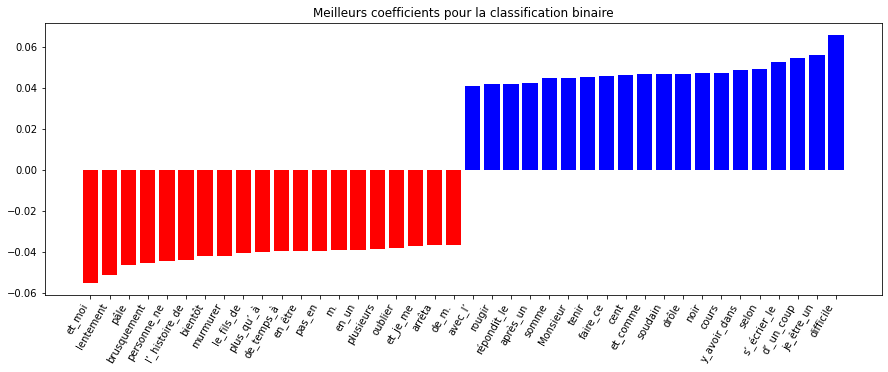
\includegraphics[width=17cm]{img/12_coef_fabula.png}
    \caption{coefficients discriminants pour le modèle, canon des auteurs}
    \label{coefs}
\end{figure}


Il est difficile d'appréhender ce qui se joue dans ces coefficients. Les mots \textit{difficile}, \textit{drôle} ou \textit{rougir} sont considérés plus canoniques que les mots \textit{pâle}, \textit{oublier} ou \textit{murmurer}. Le problème interprétatif auquel nous faisons face n'est pas dû à l'apprentissage machine mais plutôt à la complexité du phénomène que nous modélisons, la réception littéraire. Il est compliqué d'attribuer la canonicité à un groupe de mots précis, et comme nous avons fondé notre travail sur une approche linguistique avec des mots outils, nous avons en plus à interpréter des mots très courants. 

Pour comprendre ce que le modèle détecte, nous représentons dans le texte les coefficients de ce dernier. Les 500 caractéristiques les plus canoniques sont coloriés en bleu, les 500 les plus non-canoniques en rouge et le reste n'est pas représenté. Nous projetons en figure \ref{extrait_colette} ces coefficients sur un extrait de \textit{Sido}, roman écrit par Colette et publié en 1929.

\bigskip
\begin{figure}[!ht]
    \centering
    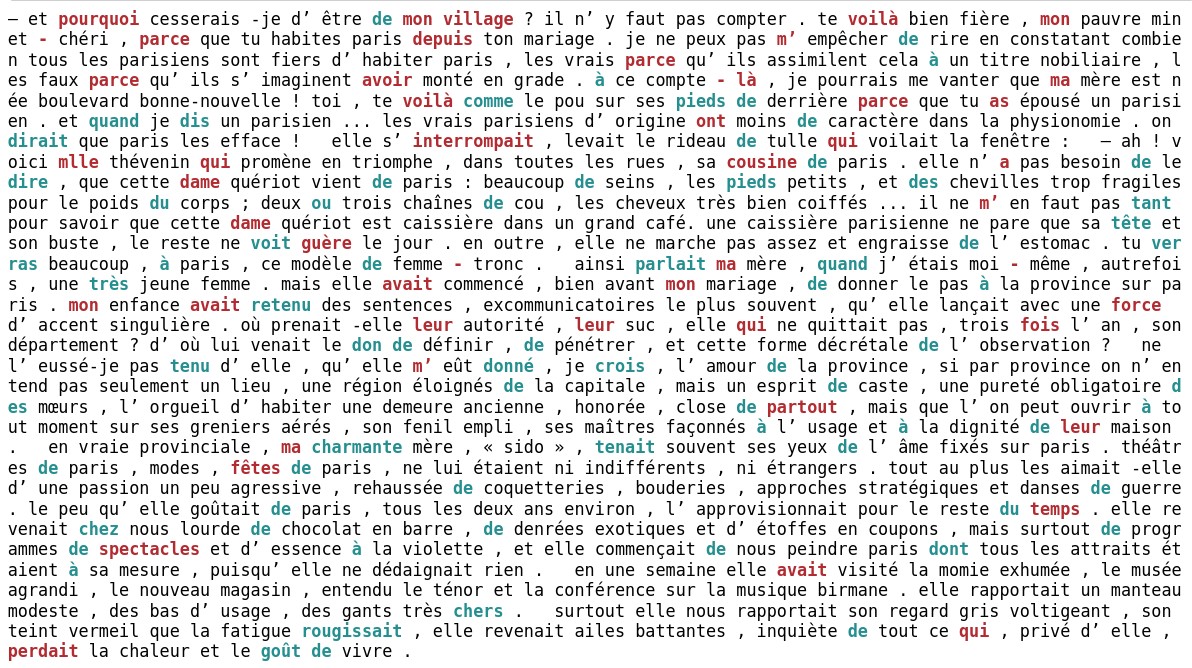
\includegraphics[width=18cm]{img/13_sido_colored.png}
    \label{extrait_colette}
    \caption{Extrait de Sido, écrit par Colette, canonicité coloriée}
\end{figure}

Dans cet extrait, nous voyons bien que le modèle ne détecte pas une manière d'être canonique. Colette écrit avec des mots considérés comme non-canonique par le modèle, comme les pronoms possessifs \textit{mon} ou \textit{ma}. Le crible du modèle statistique révèle un ensemble de traits linguistiques spécifique mais pas exclusif à ces œuvres canoniques. Le verbe \textit{rougir} ou l'adjectif qualificatif \textit{charmante} en fin d'extrait ne sont pas uniquement dédiés aux auteurs canoniques, mais le choix de ces mots est d'avantage réalisé par ces derniers.


\section{Des motifs stylistiques}

Pour palier ce problème interprétatif, nous avons revu notre démarche, avec l'objectif de détecter plus d'éléments relatifs au style. Nous avons implémenté pour cela une approche similaire à la technique des motifs stylistiques. Selon, Dominique Legallois, Thierry Charnois et Meri Larjavaara, 
\begin{displayquote}\enquote{la caractérisation du style d'un auteur, peut bénéficier d'une nouvelle d'une nouvelle méthode en linguistique de corpus, la découverte de modèles séquentiels ou de \enquote{motifs}, c'est-à-dire des chaînes contiguës de formes de mots/lemmas/POS tag. L'analyse des motifs peut être considérée comme complémentaire aux approches discrètes}\footcite{legallois_balance_2018}.
\end{displayquote}

Dans cette section, les motifs ne vont pas nous servir à caractériser un style d'auteur, mais plutôt à spécifier l'esthétique canonique que nous détectons. Nous simplifions l'approche pour construire nos motifs. On récupère de la même manière des uni-grammes, bi-grammes et tri-grammes, avec cette fois ci l'étiquetage morpho-syntaxique des mots-outils et le lemme des autres mots. 
Nous mettons le tableau des scores en annexe \ref{perf_motif}. Les résultats sont sensiblement similaires à notre première approche, ce qui s'explique par la proximité des caractéristiques textuelles utilisées. Ces résultats semblent toutefois renforcer notre première intuition : il y a bien une esthétique particulière sélectionnée dans le canon littéraire construit par nos soins. 

\bigskip
\begin{figure}[!ht]
    \centering
    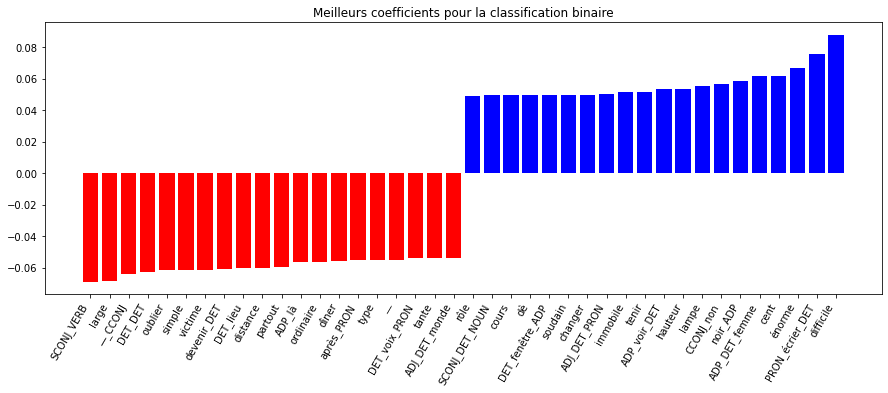
\includegraphics[width=17cm]{img/14_coefs_motifs.png}
    \caption{coefficients discriminant pour le modèle des motifs, canon des auteurs}
    \label{coefs_motifs}
\end{figure}

Dans la figure \ref{coefs_motifs} nous projetons les coefficients discriminants. On voit bien qu'en plus de mots simples, le modèle assigne de bons scores à des manières de construire une phrase. Le bi-gramme SCONJ\_VERB est la concaténation de deux mots consécutifs, en l'occurrence une conjonction de coordination avec un verbe, par exemple \enquote{Il n'est pas heureux, \textit{parce qu'habiter} en province n'est pas dans son intérêt}. Cette forme se rapproche plus selon le modèle d'une écriture non-canonique. Au contraire, le tri-gramme PRON\_écrier\_DET, qui donne par exemple\enquote{s'écria le personnage}, avec la forme pronominale du verbe écrier, est plus proche d'une écriture canonique. C'est une manière d'introduire du discours direct dans le récit, l'on ne peut pas conclure d'une utilisation plus prononcé du discours direct dans les romans canoniques avec cet unique indice.

\section{Test sur des données hors domaine d'étude}

Pour comprendre un peu mieux ce que le modèle détecte concrètement, nous lui avons donné des textes hors de son domaine d'étude pour voir quel score leur était attribué. En effet le modèle peut donner un score à tout texte écrit, même si ce n'est pas un texte littéraire. Il nous fallait des textes assez conséquents en terme de longueur, pour éviter d'avoir une matrice d'entraînement trop vide. Nous lui avons présenté deux différents textes : 

\begin{itemize}
    \item La page wikipédia du théorème de Bayes.\footnote{\url{https://fr.wikipedia.org/wiki/Théorème_de_Bayes}}
    \item Un extrait du Code Civil, le chapitre 2 du titre 2 du livre II.\footnote{\url{https://www.legifrance.gouv.fr/codes/texte_lc/LEGITEXT000006070721}}
\end{itemize}

Ce sont deux textes très formels, le premier présente une vulgarisation scientifique d'un théorème mathématique, avec une histoire et une contextualisation du théorème. L'autre comporte un chapitre du Code Civil, le tout représentant 8 articles avec de nombreux alinéas. En terme de longueur, les deux textes sont assimilables à des nouvelles suffisamment longues pour être modélisées correctement. Voici les résultats :
\bigskip

\begin{table}[ht]
    \centering
    \begin{tabular}{lrrl}
    \toprule
    {} &  proba canon &  proba non-canon & prediction \\
                     &              &                  &            \\
    \midrule
    Article du Théorème de Bayes  &         0.375779 &         0.624221 &  non\_canon \\
    Code Civil                &         0.454353 &         0.545647 &  non\_canon \\
    \bottomrule
    \end{tabular}
    \caption{Résultats des expérimentations hors domaine, canon des œuvres.}
\end{table}

Le modèle reposant sur le canon des œuvres réagit assez bien à ce test, dans le sens où il n'a l'air de reconnaître ni les traits canoniques ni ceux non-canoniques. Si les deux sont classés \enquote{non-canon}, la probabilité d'appartenance montre que le modèle n'est pas vraiment sûr de lui. Le fait que ces deux énoncés très formels soient classés comme non-canon pourrait soutenir l'idée d'un style plus développé dans le canon littéraire. 


\begin{table}[ht]
    \centering
    \begin{tabular}{lrrl}
    \toprule
    {} &  proba canon & proba non-canon &    prediction \\
                     &                  &              &             \\
    \midrule
    Article du Théorème de Bayes  &      0.484885  &    0.515115  &    non\_canon \\
    Code Civil                &      0.580976  &    0.419024  &         canon \\
    \bottomrule

    \end{tabular}
    \caption{Résultats des expérimentations hors domaine, canon des auteurs}
\end{table}

Le modèle reposant sur le canon des auteurs est lui aussi dubitatif quand à ces textes et ne sait pas comment les classer. A cette échelle le modèle se montrait très sûr de lui, et très peu de scores étaient entre 0.8 et 0.2. Cela montre bien que ces deux textes ne ressemblent en rien aux traits canoniques ou non-canoniques.

\newpage

\section{Sélectivité canonique dans la production d'un auteur}

Nos modèles détectent une filtration linguistique d'une certaine manière d'écrire des romans. Cette sélection ne se fait pas seulement au niveaux des auteurs, que l'on considère comme classique ou non, mais aussi au sein de la production littéraire d'un même auteur. Nous présentons ici les résultats des expériences menées à partir des romans de Colette, Georges Perec et Guy de Maupassant.

Pour mieux comprendre ce qui se joue à cette échelle, nous avons mis en place d'autres expériences. Avec des réductions de dimension, et plus précisément des analyses en composantes principales (ACP), nous projetons tous les ouvrages d'un même auteur sur un seul plan pour pouvoir comparer les ouvrages entre eux. 

L’ACP est une méthode bien connue de réduction de dimension qui va permettre de visualiser des données complexes pour y discerner des regroupements, des typologies. L'ACP entraîne une perte d'information car les dimensions sont réduites, mais les informations conservées sont sensées être les plus significatives.

\subsection{Colette}

\bigskip
\begin{figure}[!ht]
    \centering
    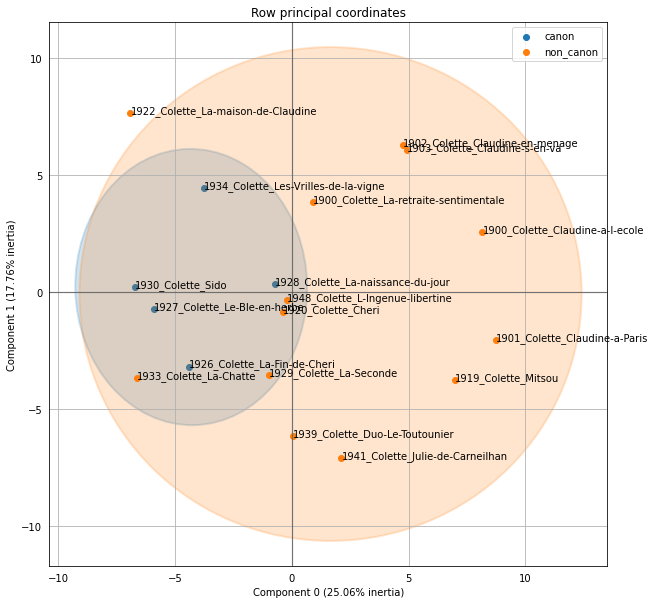
\includegraphics[width=11cm]{img/15_pca_Colette.png}
    \caption{Sélectivité canonique chez Colette}
    \label{colette}
\end{figure}

Nous avons réalisé des réductions de dimension en figure \ref{colette} sur les écrits de Colette, une écrivaine célèbre du début du XX\ieme siècle. 

Deux éléments sont mis en avant dans ce graphique, d'une part en orange les romans de Colette non-canoniques, et d'autre part en bleu les ouvrages considérés comme canoniques. On remarque que ces derniers forment un groupe assez distinct au sein de la production littéraire de Colette. L'ACP appose naturellement les romans canoniques dans la même partie du graphique, c'est à dire qu'il y a des similarités conséquentes entre ces romans. Les cinq romans canoniques sont tous écrits entre 1926 et 1934, ce qui pourrait expliquer la présence de ce groupe en tant qu'il correspond à un moment littéraire précis dans la vie de l'auteur. Loin de ce groupe se trouve la série des \textit{Claudine}, qui ont été des ouvrages très populaires mais pas intégré dans le canon. Ces ouvrages ont fait la popularité de l'auteur au début de sa carrière, mais ne correspondaient pas aux critères de sélection du canon. 


\subsection{Georges Perec}

Georges Perec est un écrivain qui a publié la majorité de ses œuvres dans la deuxième partie du XX\ieme siècle. Notre canon a retenu deux de ses ouvrages, \textit{Les choses}, publié en 1965 et \textit{La vie mode d'emploi}, publié en 1978.

\bigskip
\begin{figure}[!ht]
    \centering
    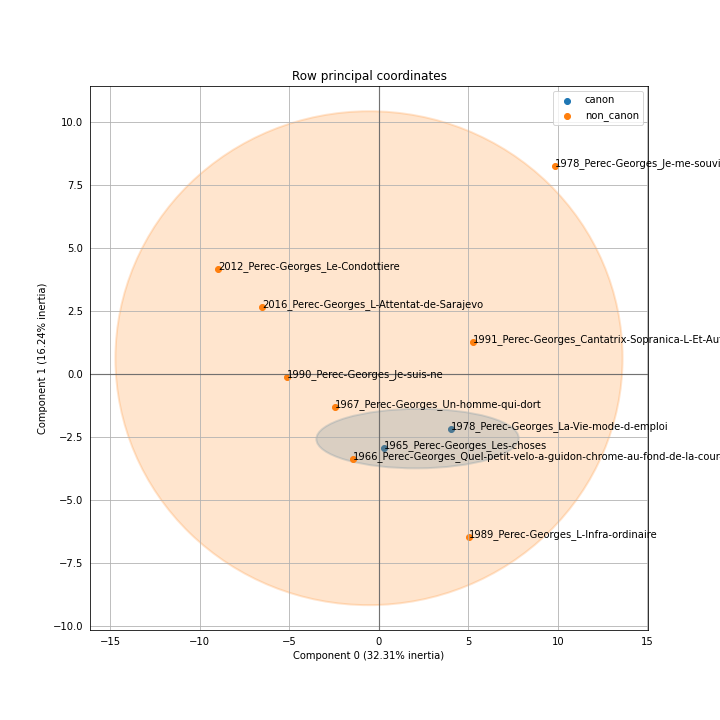
\includegraphics[width=11cm]{img/16_pca_Perec.png}
    \caption{Sélectivité canonique chez Georges Perec}
    \label{perec}
\end{figure}

L'ACP en figure \ref{perec} montre bien que ces deux ouvrages sont très similaires dans leur contenu, malgré le fait qu'ils aient été publiés à 13 années d'intervalle. Les romans acceptés dans le canon par la réception correspondent donc bien à une esthétique particulière, au sein même de la production d'un écrivain.

On remarquera que le roman \textit{Je me souviens} est très loin des autres romans, à cause de son caractère stylistiquement subversif. Le roman est un enchaînement de souvenirs de l'auteur, avec une anaphore \enquote{Je me souviens} sur tout le roman. 
C'est un roman qui a marqué la période mais il n'est pas rentré dans les critères de notre canon. 


\subsection{Guy de Maupassant}

Il est important de souligner que cette expérience ne marche pas pour tous nos auteurs. Examinons l'exemple des ouvrages de Guy de Maupassant, en figure \ref{maupa} : ce dernier est un auteur très productif, et la visualisation de la réduction de dimensionnalité ne parvient pas à séparer les canons des non-canons.

\bigskip
\begin{figure}[!ht]
    \centering
    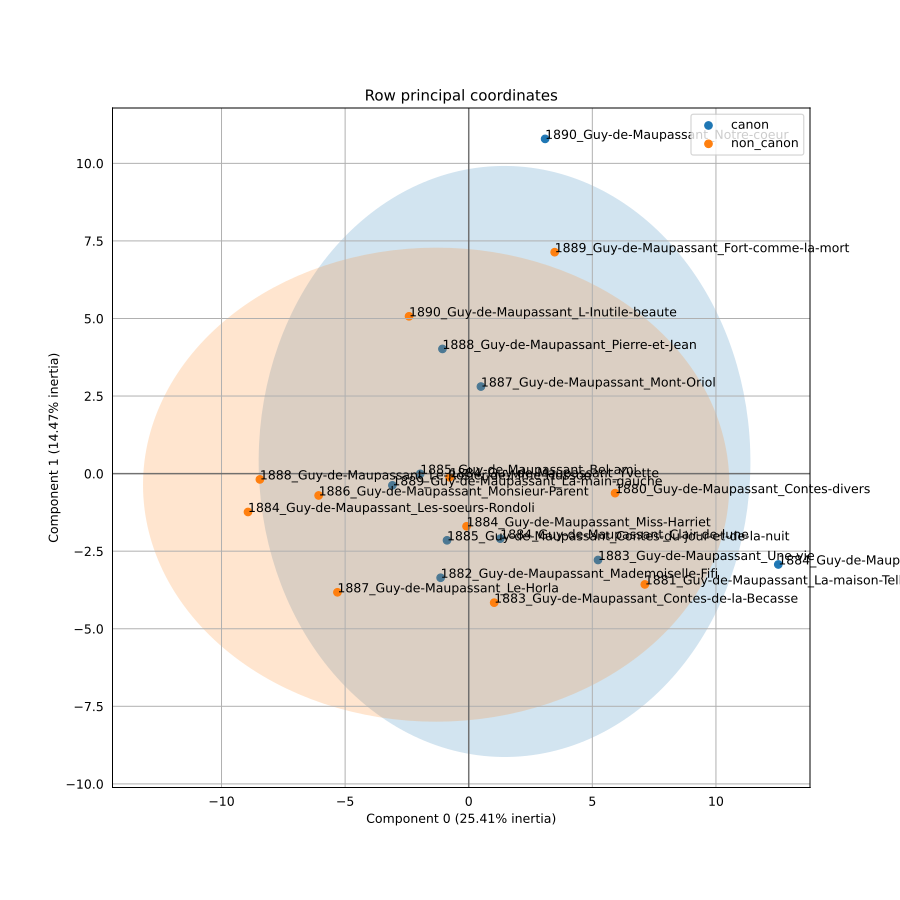
\includegraphics[width=11cm]{img/17_pca_Maupassant.png}
    \caption{Sélectivité canonique chez Maupassant}
    \label{maupa}
\end{figure}

Il y a une superposition des deux ensembles des œuvres, canoniques et non-canoniques. La critique et surtout l'institution scolaire ont tellement sacralisé le style de cet auteur que la distinction entre leurs œuvres de premier et de second plan ne tient plus, comme si le tamis sélectif avait fini par accepter la manière d'écrire de cet écrivain dans son ensemble, peu importe ses ouvrages. 

Ainsi, l'esthétique canonique constatée à l'échelle de milliers de romans par nos modèles statistiques semble sortir renforcée de nos différents tests et entrées de compréhension des données du modèle. L'étude des cas limites et les tests hors domaine d'étude semblent montrer la solidité du modèle ainsi que sa capacité à généraliser. Cette sélectivité du canon littéraire se constate aussi à l'échelle de la production d'un auteur, et ce malgré sa qualité de classique. Nos ACP montrent la filtration d'un certain type de contenu dans la production littéraire, entre un contenu conservé dans la mémoire collective et un autre laissé à l'abandon littéraire. 
\part*{Conclusion}
\addcontentsline{toc}{part}{Conclusion}
\markboth{Conclusion}{Conclusion} 

Ce travail propose une étude en profondeur de la notion de canon littéraire. Nous avons produit un ensemble de critères, fondés sur des constats historiques, pour caractériser le canon littéraire de la réception contemporaine. L'objectif de ce rapport est d'enrichir la vision traditionnelle qui envisage le  canon comme une construction arbitraire, politique, idéologique, ou relative au hasard. Nous nous sommes intéressés au contenu textuel des ouvrages pour ajouter à cette définition un aspect formel, d'ordre esthétique et interne aux œuvres qui pourrait expliquer la sélectivité du canon littéraire. À l'aide d'un grand corpus de romans, des méthodes quantitatives de l'apprentissage machine et du traitement automatique des langues, nous avons pu modéliser en lecture distante la notion de canon littéraire. Cette modélisation se fonde sur les dynamiques textuelles qui régissent les standards du jugement esthétique et la filtration institutionnelle qui en résulte.

Un des apports principaux de ce mémoire a été de montrer qu'il existait une esthétique canonique, et qu'un modèle statistique pouvait prédire la canonicité avec 75\% à 90\% d'efficacité. S'il a été difficile d'interpréter et de caractériser cette esthétique, ou de revenir à des enjeux littéraires plus concrets, nous avons pu établir les analyses suivantes : 

\begin{itemize}
    \item notre modèle détecte une usure de l'esthétique canonique dans les dernières décennies de notre histoire littéraire. On pourrait discuter de la pertinence de la notion de canon sur les décennies plus contemporaines, puisque la filtration temporelle par les différentes institutions n'a pas encore \textit{tamisé} les ouvrages.  
    \item malgré cette usure contemporaine, nous avons montré une grande stabilité du jugement esthétique sur près de deux siècles. Notre modèle a été capable de détecter des lignes structurantes bien plus stables que décrites par l'histoire littéraire. Cela pourrait s'expliquer par la seule prise en compte de la réception contemporaine. De plus amples recherches seraient nécessaires pour conclure avec certitude.
\end{itemize}

Par ailleurs, en distinguant le canon du non-canon et en décrivant ce qui rend le roman canonique singulier dans son écriture, nous avons tenté de comprendre la fonction sociale remplie par ces textes particuliers. Les éléments textuels mis à jour sont les témoins d'une manière de \textit{faire littérature}, manière sélectionnée et acceptée par la réception. Ils composent ce que l'on peut appeler un \textit{dialecte canonique}, qui est constitué d'une langue sélectionnée et autorisée dans l'enseignement, instituée comme modèle de style pour des générations d'étudiants.

Ce travail ouvre de nombreuses perspectives de recherches, d'une part pour pallier les limites de la présente étude, et d'autre part, pour préciser l'esthétique canonique détectée. Notre démarche voulait saisir quantitativement les variables linguistiques qui caractérisent le phénomène social du prestige. La tâche était d'autant plus complexe qu'elle consistait à prédire des évènements arrivés à réception, c'est-à-dire après écriture. C'est pour ces raisons que nous avons opté pour une approche simple en \textit{sac de mots}, avec un canon uniforme et des méta-données réduites. L'enjeu était de vérifier cette hypothèse de langue littéraire. Il faudrait effectuer des recherches complémentaires pour comprendre exactement ce qui se joue dans le et les canons littéraires.

Une approche future serait de récupérer des méta-données en diachronie, c'est-à-dire au fur et à mesure de la filtration de la réception. On pourrait également fragmenter notre vision du canon par acteurs du champ littéraire (éditions, manuels scolaires, prestige académique, revues littéraires, ...). Nous pourrions aussi prendre des caractéristiques textuelles plus complexes, avec des techniques algorithmiques au niveau de l'état de l'art en traitement automatique des langues, comme par exemple les vecteurs de mots ou de paragraphes, ou encore la modélisation de sujet. 

Les processus de décanonisation n'ont pas été abordés dans ce mémoire. Ils mériteraient un travail entier à eux seuls. Il faudrait identifier les ouvrages célébrés mais oubliés, qui sortent du canon au fil du temps, et étudier les raisons de cette marginalisation littéraire. 

Ainsi, notre recherche s'est inscrite dans une réflexion sur la littérature et son canon en tant qu'objet de définition d'une culture nationale. Nous avons pu mettre au jour grâce à notre démarche quantitative une norme esthétique véhiculée par le canon et entretenue par la succession des politiques culturelles. Notre diagnostic témoigne des conditions sociologiques, idéologiques et culturelles de la production de la valeur littéraire et de ses critères de sélection. Ce travail est un modeste exemple de ce que peuvent apporter les méthodes quantitatives à la recherche en sciences humaines et sociales. Les humanités numériques permettent d'ouvrir de nouvelles perspectives de compréhension du monde pour façonner des savoirs historiques inédits et comprendre les normes sociales et politiques sur lesquelles s'est construite notre société.









% annexes
\appendix
\part*{Annexes}
\addcontentsline{toc}{part}{Annexes}
\pagestyle{myheadings}
\markboth{Annexes}{Annexes}

\section{Disponibilité du code}\label{code}

Illustrations, code et données du mémoire disponibles sur Github à cette adresse : \url{https://github.com/crazyjeannot/canonization_process}. 


\newpage
\section{Le canon des auteurs}\label{canon_auteur}

\begin{xltabular}{\textwidth}{lrr}
\toprule
                    Auteurs du canon &  Nombre de romans classiques &  Nombre total de romans \\
\midrule
                    Honore De Balzac &         19 &               85 \\
                          Emile Zola &         17 &               22 \\
                      Romain Rolland &         10 &               12 \\
                   Guy De Maupassant &         10 &               21 \\
                     Alexandre Dumas &          8 &               88 \\
                         Victor Hugo &          8 &               12 \\
      François René De Chateaubriand &          7 &                7 \\
                             Colette &          5 &               18 \\
                         Jules Verne &          4 &               28 \\
                     Alphonse Daudet &          4 &               21 \\
                         George Sand &          4 &               51 \\
                            Stendhal &          4 &                7 \\
                        Albert Camus &          4 &                4 \\
         Edmond Et Jules De Goncourt &          4 &                7 \\
            Jules Barbey D'Aurevilly &          3 &                8 \\
                        Louis Aragon &          3 &                7 \\
                     Patrick Modiano &          3 &               21 \\
                    Gustave Flaubert &          3 &                7 \\
                          Jean Giono &          3 &                6 \\
                     Michel Tournier &          3 &               11 \\
                         Romain Gary &          2 &                9 \\
                     Maurice Leblanc &          2 &               33 \\
                      Claude Farrère &          2 &                5 \\
                         Michel Deon &          2 &                3 \\
                       Georges Perec &          2 &               10 \\
                        Jean Echenoz &          2 &               16 \\
                  Simone De Beauvoir &          2 &                7 \\
                    Georges Bernanos &          2 &                8 \\
                   Nathalie Sarraute &          2 &                6 \\
                 Joris Karl Huysmans &          2 &               10 \\
            Antoine De Saint Exupery &          2 &                4 \\
                       André Malraux &          2 &                3 \\
                        Jules Renard &          2 &                4 \\
                       Pierre Michon &          2 &                6 \\
                        Sainte-Beuve &          2 &                2 \\
                   Delphine De Vigan &          2 &                4 \\
                    Marguerite Duras &          2 &                8 \\
                       Laurent Gaude &          2 &                4 \\
                Marguerite Yourcenar &          2 &                9 \\
                  Maylis De Kerangal &          2 &                5 \\
                          Andre Gide &          2 &               10 \\
                        Claude Simon &          2 &               11 \\
                       Joseph Kessel &          2 &                5 \\
                        Jules Vallès &          2 &                4 \\
                 Alain Robbe-Grillet &          2 &                6 \\
                      Henri Barbusse &          2 &                2 \\
                   Théophile Gautier &          2 &                6 \\
                       Mathias Enard &          1 &                4 \\
                     Raymond Queneau &          1 &                4 \\
                       Marcel Pagnol &          1 &                7 \\
                  Frederic Beigbeder &          1 &                5 \\
                    Antoine Volodine &          1 &                9 \\
                       Emile Moselly &          1 &                2 \\
               Mme Tarbe Des Sablons &          1 &                1 \\
                      Octave Mirbeau &          1 &                5 \\
                        Henri Murger &          1 &                1 \\
                     Patrick Deville &          1 &                1 \\
           Alphonse De Chateaubriant &          1 &                2 \\
                   Philippe Grimbert &          1 &                1 \\
               Jean-Christophe Rufin &          1 &                3 \\
                        Jules  Verne &          1 &                2 \\
                     Paul Fils Feval &          1 &                6 \\
        Jean Marie Gustave Le Clézio &          1 &                4 \\
                        Marie NDiaye &          1 &                1 \\
                    Félicien Marceau &          1 &                1 \\
                      Eugène Ionesco &          1 &                1 \\
                       Henry Bauchau &          1 &                4 \\
                      Henry Bordeaux &          1 &                3 \\
                          Paul Feval &          1 &               59 \\
                       Olivier Rolin &          1 &                8 \\
                      Alain Fournier &          1 &                1 \\
                           Leon Bloy &          1 &                3 \\
                    Raymond Radiguet &          1 &                3 \\
                    Pierre Combescot &          1 &                1 \\
                              Magali &          1 &                4 \\
                        Julien Gracq &          1 &                3 \\
              Louis Ferdinand Celine &          1 &                4 \\
                   Benjamin Constant &          1 &                1 \\
                   Georges Rodenbach &          1 &                2 \\
                    Philippe Claudel &          1 &                4 \\
                   Comtesse De Segur &          1 &               11 \\
                       Michel Leiris &          1 &                1 \\
                      Marie Cardinal &          1 &                1 \\
                     Cesarie Farrenc &          1 &                1 \\
                    Emmanuel Carrere &          1 &                6 \\
                        Erik Orsenna &          1 &                1 \\
                        Albert Cohen &          1 &                1 \\
                         Marc Dugain &          1 &                1 \\
                    Christian Gailly &          1 &               10 \\
             Jean Philippe Toussaint &          1 &                2 \\
                      Samuel Beckett &          1 &                4 \\
                        Pascal Laine &          1 &                1 \\
                               Delly &          1 &               95 \\
                  Marie Darrieussecq &          1 &                8 \\
           Charles Victor Arlincourt &          1 &                7 \\
                  Michel Houellebecq &          1 &                5 \\
                       Louis Pergaud &          1 &                3 \\
                    Eugene Fromentin &          1 &                1 \\
                      Sylvie Germain &          1 &                8 \\
                       Alice Zeniter &          1 &                1 \\
                         Pierre Loti &          1 &               31 \\
                     Jacques Laurent &          1 &                6 \\
                    Didier Daeninckx &          1 &               21 \\
                       Paul Verlaine &          1 &                4 \\
                        Roger Vercel &          1 &                1 \\
                     Georges Duhamel &          1 &                5 \\
                     Pascal Quignard &          1 &               12 \\
                        Marie Nimier &          1 &                1 \\
                       Marcel Proust &          1 &                7 \\
            Emile Ajar - Gary Romain &          1 &                4 \\
                       Marcel Schwob &          1 &                2 \\
                       Pierre Benoit &          1 &                2 \\
                    Maurice Genevoix &          1 &                2 \\
                          Jean Rolin &          1 &                4 \\
                    Alfred De Musset &          1 &                2 \\
                     Alfred De Vigny &          1 &                3 \\
                       Nina Bouraoui &          1 &                7 \\
                          Paul Nizan &          1 &                3 \\
                    Mathieu Riboulet &          1 &                4 \\
                    Francois Mauriac &          1 &                1 \\
                       Louise Michel &          1 &                1 \\
                Comte De Lautreamont &          1 &                1 \\
                   Marguerite Audoux &          1 &                6 \\
                    Catherine Cusset &          1 &                2 \\
                        Annie Ernaux &          1 &                8 \\
                        Alice Ferney &          1 &                6 \\
                   Chatrian Erckmann &          1 &               20 \\
                      Paule Constant &          1 &                1 \\
\bottomrule

\end{xltabular}


\newpage


\section{Le canon des œuvres}\label{canon_roman}
\begin{xltabular}{\textwidth}{lrr}
\toprule
Date &  Auteur &Titre \\
\midrule
1811 &       Chateaubriand-François-Rene-de &                     Oeuvres-completes \\
1816 &                    Constant-Benjamin &                               Adolphe \\
1821 &            Arlincourt-Charles-Victor &                          Le-Solitaire \\
1829 &                          Hugo-Victor &         Le-dernier-jour-d-un-condamne \\
1830 &                             Stendhal &                   Le-Rouge-et-le-noir \\
1831 &                          Hugo-Victor &                   Notre-Dame-de-Paris \\
1831 &                          Hugo-Victor &                   Notre-Dame-de-Paris \\
1832 &                      Vigny-Alfred-de &                                Stello \\
1834 &                         Sainte-Beuve &                               Volupte \\
1834 &                          Hugo-Victor &                          Claude-Gueux \\
1834 &                         Sainte-Beuve &                               Volupte \\
1835 &                    Gautier-Theophile &                Mademoiselle-de-Maupin \\
1836 &                     Musset-Alfred-de &   La-Confession-d-un-enfant-du-siecle \\
1839 &                             Stendhal &                La-Chartreuse-de-Parme \\
1840 &                          Sand-George &                               Pauline \\
1842 &                     Balzac-Honore-de &                La-Femme-de-trente-ans \\
1842 &                     Balzac-Honore-de &                               Beatrix \\
1842 &                     Balzac-Honore-de &                 Le-Contrat-de-mariage \\
1843 &                      Dumas-Alexandre &                          Le-Corricolo \\
1843 &                     Balzac-Honore-de &                      Le-Cure-de-Tours \\
1843 &                     Balzac-Honore-de &                        Le-Pere-Goriot \\
1843 &                     Balzac-Honore-de &                     Illusions-perdues \\
1843 &                     Balzac-Honore-de &                             Pierrette \\
1843 &                     Balzac-Honore-de &                       Eugenie-Grandet \\
1844 &                     Balzac-Honore-de &                    Le-Colonel-Chabert \\
1844 &                     Balzac-Honore-de & Splendeurs-et-miseres-des-courtisanes \\
1844 &       Chateaubriand-François-Rene-de &                          Vie-de-Rance \\
1844 &                     Balzac-Honore-de &                 Le-Lys-dans-la-vallee \\
1844 &                      Dumas-Alexandre &               Les-Trois-Mousquetaires \\
1845 &                      Dumas-Alexandre &              Le-Comte-de-Monte-Cristo \\
1845 &                     Balzac-Honore-de &                  Un-debut-dans-la-vie \\
1845 &                     Balzac-Honore-de &                                 Adieu \\
1845 &                      Dumas-Alexandre &                       Vingt-ans-apres \\
1845 &                      Dumas-Alexandre &                       La-Reine-Margot \\
1846 &                          Sand-George &                     La-Mare-au-Diable \\
1846 &                     Balzac-Honore-de &                Physiologie-du-mariage \\
1846 &                Mme-Tarbe-Des-Sablons &                              Isabelle \\
1846 &                     Balzac-Honore-de &                         Louis-Lambert \\
1846 &                     Balzac-Honore-de &                Une-tenebreuse-affaire \\
1846 &                     Balzac-Honore-de &                    Le-Cure-de-village \\
1846 &                      Dumas-Alexandre &                  La-Dame-de-Monsoreau \\
1846 &                     Balzac-Honore-de &                Le-Medecin-de-campagne \\
1848 &                      Dumas-Alexandre &                  La-dame-aux-camelias \\
1849 &       Chateaubriand-François-Rene-de &                Memoires-d-Outre-Tombe \\
1849 &       Chateaubriand-François-Rene-de &                Memoires-d-Outre-Tombe \\
1849 &       Chateaubriand-François-Rene-de &                Memoires-d-Outre-Tombe \\
1849 &                          Sand-George &                     La-petite-Fadette \\
1849 &       Chateaubriand-François-Rene-de &                Memoires-d-Outre-Tombe \\
1849 &       Chateaubriand-François-Rene-de &                Memoires-d-Outre-Tombe \\
1850 &                      Dumas-Alexandre &              Le-Vicomte-de-Bragelonne \\
1854 &             Barbey-d-Aurevilly-Jules &                          L-ensorcelee \\
1855 &                     Balzac-Honore-de &                           Les-Paysans \\
1855 &                             Stendhal &                 Chroniques-italiennes \\
1857 &                           Feval-Paul &                              Le-Bossu \\
1857 &                     Flaubert-Gustave &                         Madame-Bovary \\
1858 &                    Segur-comtesse-de &                Les-Malheurs-de-Sophie \\
1860 &                    Erckmann-Chatrian &                   Contes-fantastiques \\
1860 &          Goncourt-Edmond-et-Jules-de &                      Charles-Demailly \\
1862 &                          Hugo-Victor &                        Les-Miserables \\
1862 &                     Flaubert-Gustave &               Salammbô \\ 
1863 &                          Verne-Jules &               Cinq-Semaines-en-ballon \\
1863 &                     Fromentin-Eugene &                             Dominique \\
1863 &                      Farrenc-Cesarie &                           La-jalousie \\
1863 &                    Gautier-Theophile &                 Le-capitaine-Fracasse \\
1864 &                          Verne-Jules &          Voyage-au-centre-de-la-Terre \\
1864 &             Barbey-d-Aurevilly-Jules &              Le-Chevalier-des-Touches \\
1864 &          Goncourt-Edmond-et-Jules-de &                    Germinie-Lacerteux \\
1864 & Goncourt-Edmond-de-Goncourt-Jules-de &                        Renee-Mauperin \\
1866 &                          Hugo-Victor &            Les-travailleurs-de-la-mer \\
1868 &                           Zola-Emile &                        Therese-Raquin \\
1869 &                          Hugo-Victor &                       L'homme-qui-rit \\
1869 &                 Lautreamont-comte-de &                Les-chants-de-Maldoror \\
1869 &                         Murger-Henri &            Scenes-de-la-vie-de-Boheme \\
1869 &                     Flaubert-Gustave & L'education-sentimentale \\  
1870 &                           Zola-Emile &                 La-fortune-des-Rougon \\
1870 &                          Verne-Jules &      Vingt-mille-lieues-sous-les-mers \\
1872 &                           Zola-Emile &                              La-curee \\
1873 &                           Zola-Emile &                    Le-ventre-de-Paris \\
1873 &                      Daudet-Alphonse &                       Contes-du-lundi \\
1874 &                     Flaubert-Gustave &         La-tentation-de-saint-Antoine \\
1874 &                          Hugo-Victor &                    Quatrevingt-Treize \\
1874 &             Barbey-d-Aurevilly-Jules &                       Les-Diaboliques \\
1875 &                      Daudet-Alphonse &                                  Jack \\
1875 &                           Zola-Emile &             La-faute-de-l-abbe-Mouret \\
1876 &                           Zola-Emile &          Son-excellence-Eugene-Rougon \\
1876 &                          Sand-George &                                Horace \\
1877 &          Goncourt-Edmond-et-Jules-de &                   La-fille-Elisa \\
1877 &                     Flaubert-Gustave &                  Trois contes \\
1878 &                          Verne-Jules &            Un-capitaine-de-quinze-ans \\
1878 &                           Zola-Emile &                       Madeleine-Ferat \\
1879 &                  Huysmans-Joris-Karl &                     Les-soeurs-Vatard \\
1879 &                      Daudet-Alphonse &                 Lettres-de-mon-moulin \\
1880 &                           Zola-Emile &                                  Nana \\
1881 &                         Valles-Jules &                          Le-Bachelier \\
1881 &                         Valles-Jules &                              L-Enfant \\
1881 &                     Flaubert-Gustave &                   Bouvard-et-Pecuchet \\
1882 &                    Guy-de-Maupassant &                     Mademoiselle-Fifi \\
1883 &                           Zola-Emile &                  Au-bonheur-des-dames \\
1883 &                    Guy-de-Maupassant &                               Une-vie \\
1884 &                           Zola-Emile &                      La-joie-de-vivre \\
1884 &                    Guy-de-Maupassant &                         Clair-de-lune \\
1884 &                      Daudet-Alphonse &                                 Sapho \\
1884 &                  Huysmans-Joris-Karl &                             a-rebours \\
1884 &                    Guy-de-Maupassant &                             Au-soleil \\
1885 &                           Zola-Emile &                              Germinal \\
1885 &                          Verne-Jules &                       Mathias-Sandorf \\
1885 &                    Guy-de-Maupassant &                               Bel-ami \\
1885 &                    Guy-de-Maupassant &          Contes-du-jour-et-de-la-nuit \\
1886 &                        Michel-Louise &                              Memoires \\
1887 &                           Zola-Emile &                              La-terre \\
1887 &                            Bloy-Leon &                          Le-Desespere \\
1887 &                    Guy-de-Maupassant &                            Mont-Oriol \\
1887 &                          Loti-Pierre &                   Madame-Chrysantheme \\
1888 &                           Zola-Emile &                               Le-reve \\
1888 &                    Guy-de-Maupassant &                        Pierre-et-Jean \\
1889 &                    Guy-de-Maupassant &                        La-main-gauche \\
1890 &                    Guy-de-Maupassant &                           Notre-coeur \\
1890 &                           Zola-Emile &                       La-bete-humaine \\
1891 &                           Zola-Emile &                              L-argent \\
1892 &                           Zola-Emile &                            La-debacle \\
1892 &                    Rodenbach-Georges &                       Bruges-la-Morte \\
1893 &                           Zola-Emile &                     Le-docteur-Pascal \\
1893 &                        Verlaine-Paul &                           Mes-prisons \\
1893 &                         Renard-Jules &                          Coquecigrues \\
1893 &                      Leblanc-Maurice &                             Une-femme \\
1894 &                         Renard-Jules &                       Poil-de-carotte \\
1894 &                             Stendhal &                         Lucien-Leuwen \\
1895 &                      Leblanc-Maurice &                                Contes \\
1896 &                        Schwob-Marcel &                      Vies-imaginaires \\
1900 &                       Mirbeau-Octave &     Le-journal-d-une-femme-de-chambre \\
1904 &                       Rolland-Romain &                       Jean-Christophe \\
1904 &                       Rolland-Romain &                       Jean-Christophe \\
1904 &                       Rolland-Romain &                       Jean-Christophe \\
1905 &                       Rolland-Romain &                       Jean-Christophe \\
1905 &                       Farrere-Claude &                         Les-civilises \\
1907 &                        Moselly-Emile &                      Terres-lorraines \\
1908 &                       Rolland-Romain &                       Jean-Christophe \\
1908 &                       Barbusse-Henri &                               L-enfer \\
1908 &                       Rolland-Romain &                       Jean-Christophe \\
1908 &                       Rolland-Romain &                       Jean-Christophe \\
1909 &                       Farrere-Claude &                           La-Bataille \\
1910 &                    Audoux-Marguerite &                          Marie-Claire \\
1910 &                       Rolland-Romain &                       Jean-Christophe \\
1911 &                       Rolland-Romain &                       Jean-Christophe \\
1912 &                        Pergaud-Louis &                 La-Guerre-des-boutons \\
1912 &                       Rolland-Romain &                       Jean-Christophe \\
1913 &                       Bordeaux-Henry &                             La-Maison \\
1913 &                       Alain-Fournier &                     Le-grand-Meaulnes \\
1914 &                           Gide-Andre &                  Les-Caves-du-Vatican \\
1916 &                       Barbusse-Henri &                                Le-Feu \\
1919 &                        Benoit-Pierre &                           L-Atlantide \\
1922 &                         Aragon-Louis &            Les-aventures-de-Telemaque \\
1922 &                      Feval-Paul-fils &                              Le-Bossu \\
1923 &                     Radiguet-Raymond &                    Le-diable-au-corps \\
1923 &            Chateaubriant-Alphonse-de &                             La-Briere \\
1925 &                     Genevoix-Maurice &                              Raboliot \\
1925 &                        Proust-Marcel &                    Albertine-disparue \\
1926 &                     Bernanos-Georges &               Sous-le-soleil-de-Satan \\
1926 &                              Colette &                       La-Fin-de-Cheri \\
1926 &                        Kessel-Joseph &                           Les-Captifs \\
1927 &                              Colette &                       Le-Ble-en-herbe \\
1927 &                           Gide-Andre &                   Les-Faux-monnayeurs \\
1928 &                              Colette &                  La-naissance-du-jour \\
1929 &                     Bernanos-Georges &                               La-joie \\
1930 &                           Giono-Jean &                                Regain \\
1930 &                        Malraux-Andre &                        La-voie-royale \\
1930 &                              Colette &                                  Sido \\
1931 &             Saint-Exupery-Antoine-de &                           Vol-de-nuit \\
1932 &               Celine-Louis-Ferdinand &             Voyage-au-bout-de-la-nuit \\
1933 &                      Duhamel-Georges &                   Le-notaire-du-Havre \\
1933 &                        Malraux-Andre &                  La-Condition-Humaine \\
1934 &                         Vercel-Roger &                       Capitaine-Conan \\
1934 &                              Colette &               Les-Vrilles-de-la-vigne \\
1935 &                                Delly &                                Contes \\
1936 &                         Aragon-Louis &                   Les-Beaux-Quartiers \\
1936 &                           Giono-Jean &                  Les-vraies-richesses \\
1938 &                           Nizan-Paul &                       La-Conspiration \\
1939 &             Saint-Exupery-Antoine-de &                      Terre-des-hommes \\
1939 &                    Sarraute-Nathalie &                             Tropismes \\
1939 &                        Leiris-Michel &                         L-Age-d-homme \\
1942 &                         Camus-Albert &                            L-etranger \\
1944 &                         Camus-Albert &                      Le-premier-homme \\
1947 &                         Camus-Albert &                              La-peste \\
1950 &                     Duras-Marguerite &        Un-barrage-contre-le-Pacifique \\
1951 &                         Gracq-Julien &                  Le-rivage-des-Syrtes \\
1951 &                           Giono-Jean &                Le-Hussard-sur-le-toit \\
1951 &                       Beckett-Samuel &                                Molloy \\
1953 &                  Robbe-Grillet-Alain &                            Les-Gommes \\
1954 &                         Cohen-Albert &                   Le-livre-de-ma-mere \\
1954 &                   Beauvoir-Simone-de &                         Les-Mandarins \\
1954 &                   Beauvoir-Simone-de &                         Les-Mandarins \\
1956 &                          Gary-Romain &                   Les-Racines-du-Ciel \\
1958 &                        Kessel-Joseph &                               Le-lion \\
1959 &                      Queneau-Raymond &                   Zazie-Dans-Le-Metro \\
1960 &                        Pagnol-Marcel &                  Le-Temps-des-Secrets \\
1960 &                          Gary-Romain &                 La-promesse-de-l-aube \\
1960 &                         Simon-Claude &                 La-Route-des-Flandres \\
1965 &                        Perec-Georges &                            Les-choses \\
1967 &                      Tournier-Michel &   Vendredi-ou-les-limbes-du-Pacifique \\
1967 &                         Simon-Claude &                              Histoire \\
1968 &                 Yourcenar-Marguerite &                      L-Oeuvre-Au-Noir \\
1969 &                               Magali &                        La-prisonniere \\
1969 &                     Mauriac-Francois &             Un-adolescent-d-autrefois \\
1969 &                     Marceau-Felicien &                                Creezy \\
1970 &                          Deon-Michel &                   Les-poneys-sauvages \\
1970 &                      Tournier-Michel &                     Le-Roi-des-Aulnes \\
1971 &                      Laurent-Jacques &                           Les-betises \\
1971 &                      Tournier-Michel &            Vendredi-ou-la-vie-sauvage \\
1972 &                         Aragon-Louis &                              Aurelien \\
1972 &                      Modiano-Patrick &            Les-boulevards-de-ceinture \\
1973 &                          Deon-Michel &                         Un-Taxi-mauve \\
1973 &                       Ionesco-Eugene &                          Le-solitaire \\
1974 &                         Laine-Pascal &                        La-dentelliere \\
1974 &                 Yourcenar-Marguerite &                       Souvenirs-pieux \\
1975 &                       Cardinal-Marie &                 Les-mots-pour-le-dire \\
1975 &               Ajar-Emile-Gary-Romain &                     La-Vie-Devant-Soi \\
1977 &                      Modiano-Patrick &                     Livret-de-famille \\
1978 &                      Modiano-Patrick &            Rue-des-boutiques-obscures \\
1978 &                        Perec-Georges &                  La-Vie-mode-d-emploi \\
1980 &         Le-Clezio-Jean-Marie-Gustave &                                Desert \\
1983 &                    Sarraute-Nathalie &                               Enfance \\
1983 &                         Ernaux-Annie &                              La-place \\
1983 &                         Echenoz-Jean &                              Cherokee \\
1984 &                     Duras-Marguerite &                               L-Amant \\
1988 &                         Orsenna-Erik &                L-exposition-coloniale \\
1991 &                      Quignard-Pascal &              Tous-Les-Matins-Du-Monde \\
1991 &                        Michon-Pierre &                       Rimbaud-le-fils \\
1991 &                     Combescot-Pierre &                Les-filles-du-Calvaire \\
1994 &                         Camus-Albert &                      Le-premier-homme \\
1994 &                        Rolin-Olivier &                           Port-Soudan \\
1995 &                     Carrere-Emmanuel &                    La-classe-de-neige \\
1996 &                           Rolin-Jean &                        L-Organisation \\
1998 &                       Constant-Paule &            Confidence-pour-confidence \\
1998 &                          Dugain-Marc &              La-chambre-des-officiers \\
1998 &                     Daeninckx-Didier &                             Cannibale \\
1999 &                     Volodine-Antoine &                     Des-anges-mineurs \\
1999 &                         Echenoz-Jean &                          Je-m-en-vais \\
2001 &                  Robbe-Grillet-Alain &                            La-reprise \\
2001 &                        Gaude-Laurent &                                  Cris \\
2001 &                     Gailly-Christian &                       Un-soir-au-club \\
2001 &                Rufin-Jean-Christophe &                          Rouge-Bresil \\
2002 &                        Gaude-Laurent &                La-Mort-du-roi-Tsongor \\
2003 &                   Beigbeder-Frederic &                  Windows-on-the-World \\
2004 &                    Grimbert-Philippe &                             Un-secret \\
2005 &                       Germain-Sylvie &                                Magnus \\
2005 &                        Bouraoui-Nina &                 Mes-mauvaises-pensees \\
2006 &                         Nimier-Marie &                   La-Reine-du-silence \\
2007 &                    de-Vigan-Delphine &                             No-et-moi \\
2007 &                     Claudel-Philippe &                 Le-rapport-de-Brodeck \\
2008 &                        Enard-Mathias &                                  Zone \\
2008 &                        Bauchau-Henry &             Le-Boulevard-peripherique \\
2008 &                     Cusset-Catherine &                    Un-brillant-avenir \\
2009 &              Toussaint-Jean-Philippe &                   La-Verite-sur-Marie \\
2009 &                    Vigan-Delphine-de &               Les-heures-souterraines \\
2009 &                        Michon-Pierre &                              Les-Onze \\
2009 &                        N-Diaye-Marie &               Trois-femmes-puissantes \\
2010 &                   Kerangal-Maylis-de &                   Naissance-d-un-pont \\
2010 &                   Houellebecq-Michel &             La-Carte-et-le-territoire \\
2012 &                     Riboulet-Mathieu &            Les-oeuvres-de-misericorde \\
2012 &                      Deville-Patrick &                      Peste-et-cholera \\
2013 &                        Zeniter-Alice &                       Sombre-dimanche \\
2013 &                         Ferney-Alice &                     Cherchez-La-Femme \\
2013 &                   Darrieussecq-Marie &     Il-faut-beaucoup-aimer-les-hommes \\
2014 &                   Kerangal-Maylis-de &                   Reparer-les-vivants \\
\bottomrule
\end{xltabular}


\newpage
\section{Scores des motifs stylistiques}\label{perf_motif}

	\begin{table}[ht]
		\centering % Centre the table on the slide
		\begin{tabular}{l c c c c c}
			\toprule
    			 & precision & recall & f1-score & support & accuracy \\
			\toprule
			canon & 0.868 & 0.886 & 0.878 & 230 \\
			\midrule
			non-canon & 0.928 & 0.912 & 0.916 & 361 \\
			\midrule
			full dataset & & & & 592 & \textbf{0.902}\\
			\midrule
			macro-average & 0.896 & 0.898 & 0.896 & 591 \\
			\midrule
			weighted average & 0.902 & 0.898 & 0.902 & 591 \\

			\bottomrule
		\end{tabular}
	\caption{Résultats de l'évaluation du modèle en validation croisée pour les motifs}
	\end{table} 


\newpage 
\section{Passage remarquable dans \textit{L'éducation sentimentale}, de Gustave Flaubert}\label{eds}

Le souci de la vérité extérieure dénote la bassesse contemporaine ; et l’art deviendra, si l’on continue, je ne sais quelle rocambole au-dessous de la religion comme poésie, et de la politique comme intérêt. Vous n’arriverez pas à son but, – oui, son but ! – qui est de nous causer une exaltation impersonnelle, avec de petites œuvres, malgré toutes vos finasseries d’exécution. Voilà les tableaux de Bassolier, par exemple : c’est joli, coquet, propret, et pas lourd ! Ça peut se mettre dans la poche, se prendre en voyage ! Les notaires achètent ça vingt mille francs ; il y a pour trois sous d’idées ; mais, sans l’idée, rien de grand ! sans grandeur, pas de beau ! L’Olympe est une montagne ! Le plus crâne monument, ce sera toujours les Pyramides. Mieux vaut l’exubérance que le goût, le désert qu’un trottoir, et un sauvage qu’un coiffeur ! Frédéric, en écoutant ces choses, regardait Mme Arnoux. Elles tombaient dans son esprit comme des métaux dans une fournaise, s’ajoutaient à sa passion et faisaient de l’amour. Il était assis trois places au-dessous d’elle, sur le même côté. De temps à autre, elle se penchait un peu, en tournant la tête pour adresser quelques mots à sa petite fille ; et, comme elle souriait alors, une fossette se creusait dans sa joue, ce qui donnait à son visage un air de bonté plus délicate.Au moment des liqueurs, elle disparut. La conversation devint très libre ; M. Arnoux y brilla, et Frédéric fut étonné du cynisme de ces hommes. Cependant, leur préoccupation de la femme établissait entre eux et lui comme une égalité, qui le haussait dans sa propre estime. Rentré au salon, il prit, par contenance, un des albums traînant sur la table. Les grands artistes de l’époque l’avaient illustré de dessins, y avaient mis de la prose, des vers, ou simplement leurs signatures ; parmi les noms fameux, il s’en trouvait beaucoup d’inconnus, et les pensées curieuses n’apparaissaient que sous un débordement de sottises. Toutes contenaient un hommage plus ou moins direct à Mme Arnoux. Frédéric aurait eu peur d’écrire une ligne à côté. Elle alla chercher dans son boudoir le coffret à fermoirs d’argent qu’il avait remarqué sur la cheminée. C’était un cadeau de son mari, un ouvrage de la Renaissance. Les amis d’Arnoux le complimentèrent, sa femme le remerciait ; il fut pris d’attendrissement, et lui donna devant le monde un baiser. Ensuite, tous causèrent çà et là, par groupes ; le bonhomme Meinsius était avec Mme Arnoux, sur une bergère, près du feu ; elle se penchait vers son oreille, leurs têtes se touchaient ; et Frédéric aurait accepté d’être sourd, infirme et laid pour un nom illustre et des cheveux blancs, enfin pour avoir quelque chose qui l’intronisât dans une intimité pareille. Il se rongeait le cœur, furieux contre sa jeunesse. Mais elle vint dans l’angle du salon où il se tenait, lui demanda s’il connaissait quelques-uns des convives, s’il aimait la peinture, depuis combien de temps il étudiait à Paris. Chaque mot qui sortait de sa bouche semblait à Frédéric être une chose nouvelle, une dépendance exclusive de sa personne.

\newpage 
\section{Passage remarquable dans \textit{Un petit monde d'enfants}, de Elise Pressense}\label{enfants}

 — Maurice, tu oublies que je suis seule pour suffire à tout et que je suis moins forte qu’autrefois.  Il ne répondit pas et la mère continua :  —Oh ! mon pauvre enfant, si tu voulais m’écouter et te donner de la peine pour apprendre à lire et à écrire !... Tu es grand et fort ; l’année prochaine tu entrerais en apprentissage et tu pourrais bientôt m’aider. Pense comme tu serais heureux quand tu m apporterais l’argent que tu aurais gagné toi-même, et comme alors tout deviendrait facile.  Maurice balançait ses pieds sans répondre et tenait sa tête baissée pour ne pas rencontrer le regard de sa mère. Quelque chose lui disait qu’il serait en effet bien heureux de gagner de l’argent et de le lui donner, mais pour rien au monde il n’aurait voulu lui faire le plaisir d’en convenir. Il ne voulait pas la regarder non plus, car il sentait que peut-être il lui serait plus difficile de résister au muet appel de ses yeux qu’à ses paroles. Il se leva pour quitter la chambre.  — Ne vas-tu pas à l’école du dimanche ? demanda Madame Richard.  — Non, répondit-il en avançant un pied, puis l’autre. Je ne veux pas y aller avec ces souliers-là. Ça prend l’eau comme une éponge.  — Mais tu vas bien courir dans la neige.  Maurice ne répondit pas, et ferma la porte sur lui avec un bruit qui fit tressaillir tous les voisins dans leurs chambres.  Madame Richard, restée seule, pleura longtemps. Elle se sentait si faible, si seule, et l’égoïsme de son enfant lui faisait tant de mal ! Que n’avait-elle pas fait pour lui ! Que de nuits sans sommeil, que de journées de travail fiévreux ! Que de retranchements sur son strict nécessaire, à elle, pour donner à l’enfant un plaisir de plus ! Hélas ! elle le savait bien, elle l’avait gâté, et maintenant, elle recueillait les fruits amers de sa faiblesse.  Maurice descendit dans la cour, rendez-vous ordinaire de ses camarades. La neige tombée la veille avait été balayée et formait un amas grisâtre dans un coin. Les moineaux affamés sautillaient jusque sur le seuil de la porte, dans l’espoir d’y trouver quelques miettes de pain ; le soleil brillait, mais sans réchauffer, et les branches les plus déliées d’un arbre dont le sommet dépouillé apparaissait derrière un haut mur, se dessinaient avec une netteté parfaite contre le ciel, d’un bleu froid.  Maurice regarda les rangées d’innombrables fenêtres qui donnaient sur la cour. Tout était bien clos, personne ne songeait à mettre le nez dehors ; on n’entendait ni cris ni éclats de rire ; on eût dit que tous les habitants de la grande maison noire se livraient au repos du dimanche.  Cependant une petite figure, ensevelie dans un immense capuchon, parut sur le pas de la porte, et, toute frissonnante, s’y arrêta pour regarder les moineaux. Lydie avait un peu de pain dans sa poche ; elle le leur émietta, et les oisillons se mirent à voleter et à becqueter autour d’elle, tout ravis de ce festin inattendu.



\newpage 
\section{Projet ANR « Chapitres (XIXe-XXe siècles) »}\label{chapitre}

\bigskip

Je remercie toute l'équipe de l'ANR Chapitres et en particulier Aude Leblond pour m'avoir permis de réaliser mes recherches sur leur corpus. 

\bigskip

\textbf{Équipe de l'ANR Chapitres :}
\begin{itemize}
    \item Aude Leblond
    \item Claire Colin
    \item Thomas Conrad
    \item Marianne Reboul
    \item Raphaël Baroni
    \item Alexandre Gefen
    \item Camille Koskas
    \item Virginie Tahar
    \item Michel Bernard
    \item Alain Schaffner
    \item Jérémy Naïm
    \item Ugo Dionne
    \item Dimitri Garncarzyk
    \item Anaïs Goudmand
    \item Victoire Feuillebois
\end{itemize}

\bigskip

Lien : \url{https://chapitres.hypotheses.org/}.

\bigskip


Publication principale : \enquote{Pratique et poétiques du chapitre du XIXe au XXIe siècle}\footcites{colin_pratiques_2017}.
\backmatter

\addcontentsline{toc}{chapter}{Bibliographie}
%\nocite{*}
\printbibliography

% glossaire
%\include{back/glossaire}

% Liste des figures
\listoffigures
% table des tableaux
\listoftables


\end{document}